\documentclass[11pt]{article}
\usepackage[utf8]{inputenc}
\usepackage{amsmath, amssymb, dsfont}
\usepackage{titling, fancyhdr, authblk}
\usepackage{algorithm, algpseudocode}
\usepackage{graphicx, epsfig, xcolor, subfig}
\usepackage{float}
\usepackage{indentfirst}
\usepackage{setspace}
\usepackage{enumitem}
\usepackage{caption}
\usepackage{hyperref}
\usepackage{pdfpages}
\usepackage{soul}
\usepackage{booktabs}
\usepackage{style}
\usepackage{adjustbox}
\usepackage{longtable}
\usepackage[backend=bibtex, style=alphabetic]{biblatex}
\addbibresource{bibliography.bib}
\usepackage[a4paper,margin=1in]{geometry}
\usepackage{minted}

\pagestyle{fancy}
\fancyhf{}
\lhead{Team 01}
\rhead{\thepage}
\renewcommand{\footrulewidth}{0pt}
\newcommand{\note}[1]{{\Large \hl{#1}}}

\setboolean{@twoside}{false}

\begin{document}

\begin{titlepage}
    \centering
    \vfill
    \epsfig{file=brownlogo.eps, height=1.0in, width=2.0in}
    \vskip4cm
    {\large Brown Mathematical Contest for Modeling 2022}
    \vskip4cm
    {\textbf{\Large
    Combating Urban Heat Islands with Strategic Vegetation
    }}
    \vskip.5cm
    {\Large A Case Study on Durham, NC}
    \vskip3cm
    Hyoungjin Kim\qquad Benjamin Shih\qquad Alexander Zheng
    \vskip3cm
    Department of Applied Mathematics  \\
    Brown University \\
    \texttt{\{hyoungjin\_kim, benjamin\_shih, alexander\_zheng\}@brown.edu}
    \vfill
\end{titlepage}

\tableofcontents

\section{Introduction}
\subsection{Problem Explanation}
The issue of global warming has been recognized for decades by scientists, and since the turn of the century, increasingly so by the general public as well. However, the increased awareness has not translated into meaningful and effective solutions.

Both the lack of decisive action at a government level and a sense of ``one person isn't going to make a difference" at an individual level has kept us on a trajectory of ever-increasing temperature records. This has only been exacerbated by coverage of such "records" by various outlets as simple milestones to be reached, numbing the public to the real and personal effects of global warming.

Then, given our historical inability as a people to take impactful action at a larger scale, it is critical that communities and governments at a more localized level work to at least mitigate the impacts of global warming. A particular phenomenon that we can seek to address is the Urban Heat Island effect.

\subsection{Existing Literature}
The Urban Heat Island effect represents the phenomenon of modern city construction trapping excess heat throughout the day, then releasing the heat at night. Specifically, the effect is brought about by common construction materials, such as concrete and cement on roads and sidewalks, as well as clay and metal used in housing and roofing \cite{kim_2007}. These materials, although great for building with, have the unfortunate downside of being excellent trappers of heat.

The prevalence of these materials in urban and suburban areas keeps temperatures elevated even during the cooler night hours, especially in the summer months. The result is that the eventual consequences of global warming, such as heat-related illnesses and associated hospitalizations, are exacerbated.

One potential solution to UHI is the use of trees and vegetation to reduce temperatures. Research indicates that higher levels of vegetation, especially in the form of trees, are effective at reducing temperatures \cite{osti_10180633}.

As an extension, additional research indicates that planting trees may be a cost-effective solution to UHI consequences. By reducing hospitalization rates for heat-related illnesses, the planting of trees can actually help cities save money in the long run \cite{mcpherson_simpson_peper_maco_xiao_2005}.

We now note that vegetation appears to be a potentially effective solution in combating UHI. The remainder of this paper will then assume planting vegetation as a viable solution method. With this is mind, we will instead turn our attention to the question of how a city may be able to most effectively utilize green spaces as a means to alleviate the temperature elevations cause by UHI.

\subsection{Problem Restatement}
\noindent The goal of this paper is then to address the following:
\begin{enumerate}
    \item Explore trends in Durham's demographic, geographic, and meteorological data to determine the interactions between the features
    \item Apply these interactions to create a model that optimally allocates a limited project budget to census tracts for greenery development
    \item Identify a metric for utility per dollar efficiency with the goal of advising decision-makers with a recommendation of the optimal project budget
\end{enumerate}
\pagebreak

\section{Initial Exploration}
The data set provided described 193 measurements of nighttime temperature reduction throughout Durham, North Carolina. In conjunction with these mentions, the data set indicated the corresponding percent below two times the poverty level, percent green coverage, and latitude-longitude coordinates. In the following sections, we discuss the results of the initial exploratory analysis we conducted which revealed several trends critical to our core modeling work.

\subsection{Spatial Relations}
Given a data set of measurements associated with coordinates, we investigated geographic patterns within the data ranging from the distribution of city tracts themselves to geographic relations with temperature and greenery coverage. Preliminary analysis of spatial trends and underlying patterns gives way to important modeling decisions later on.

\subsubsection{Location Frequency}
First, we generated a kernel density estimation from the given coordinates along with the marginal distributions of longitudes and latitudes.

\begin{figure}[H]
    \centering
    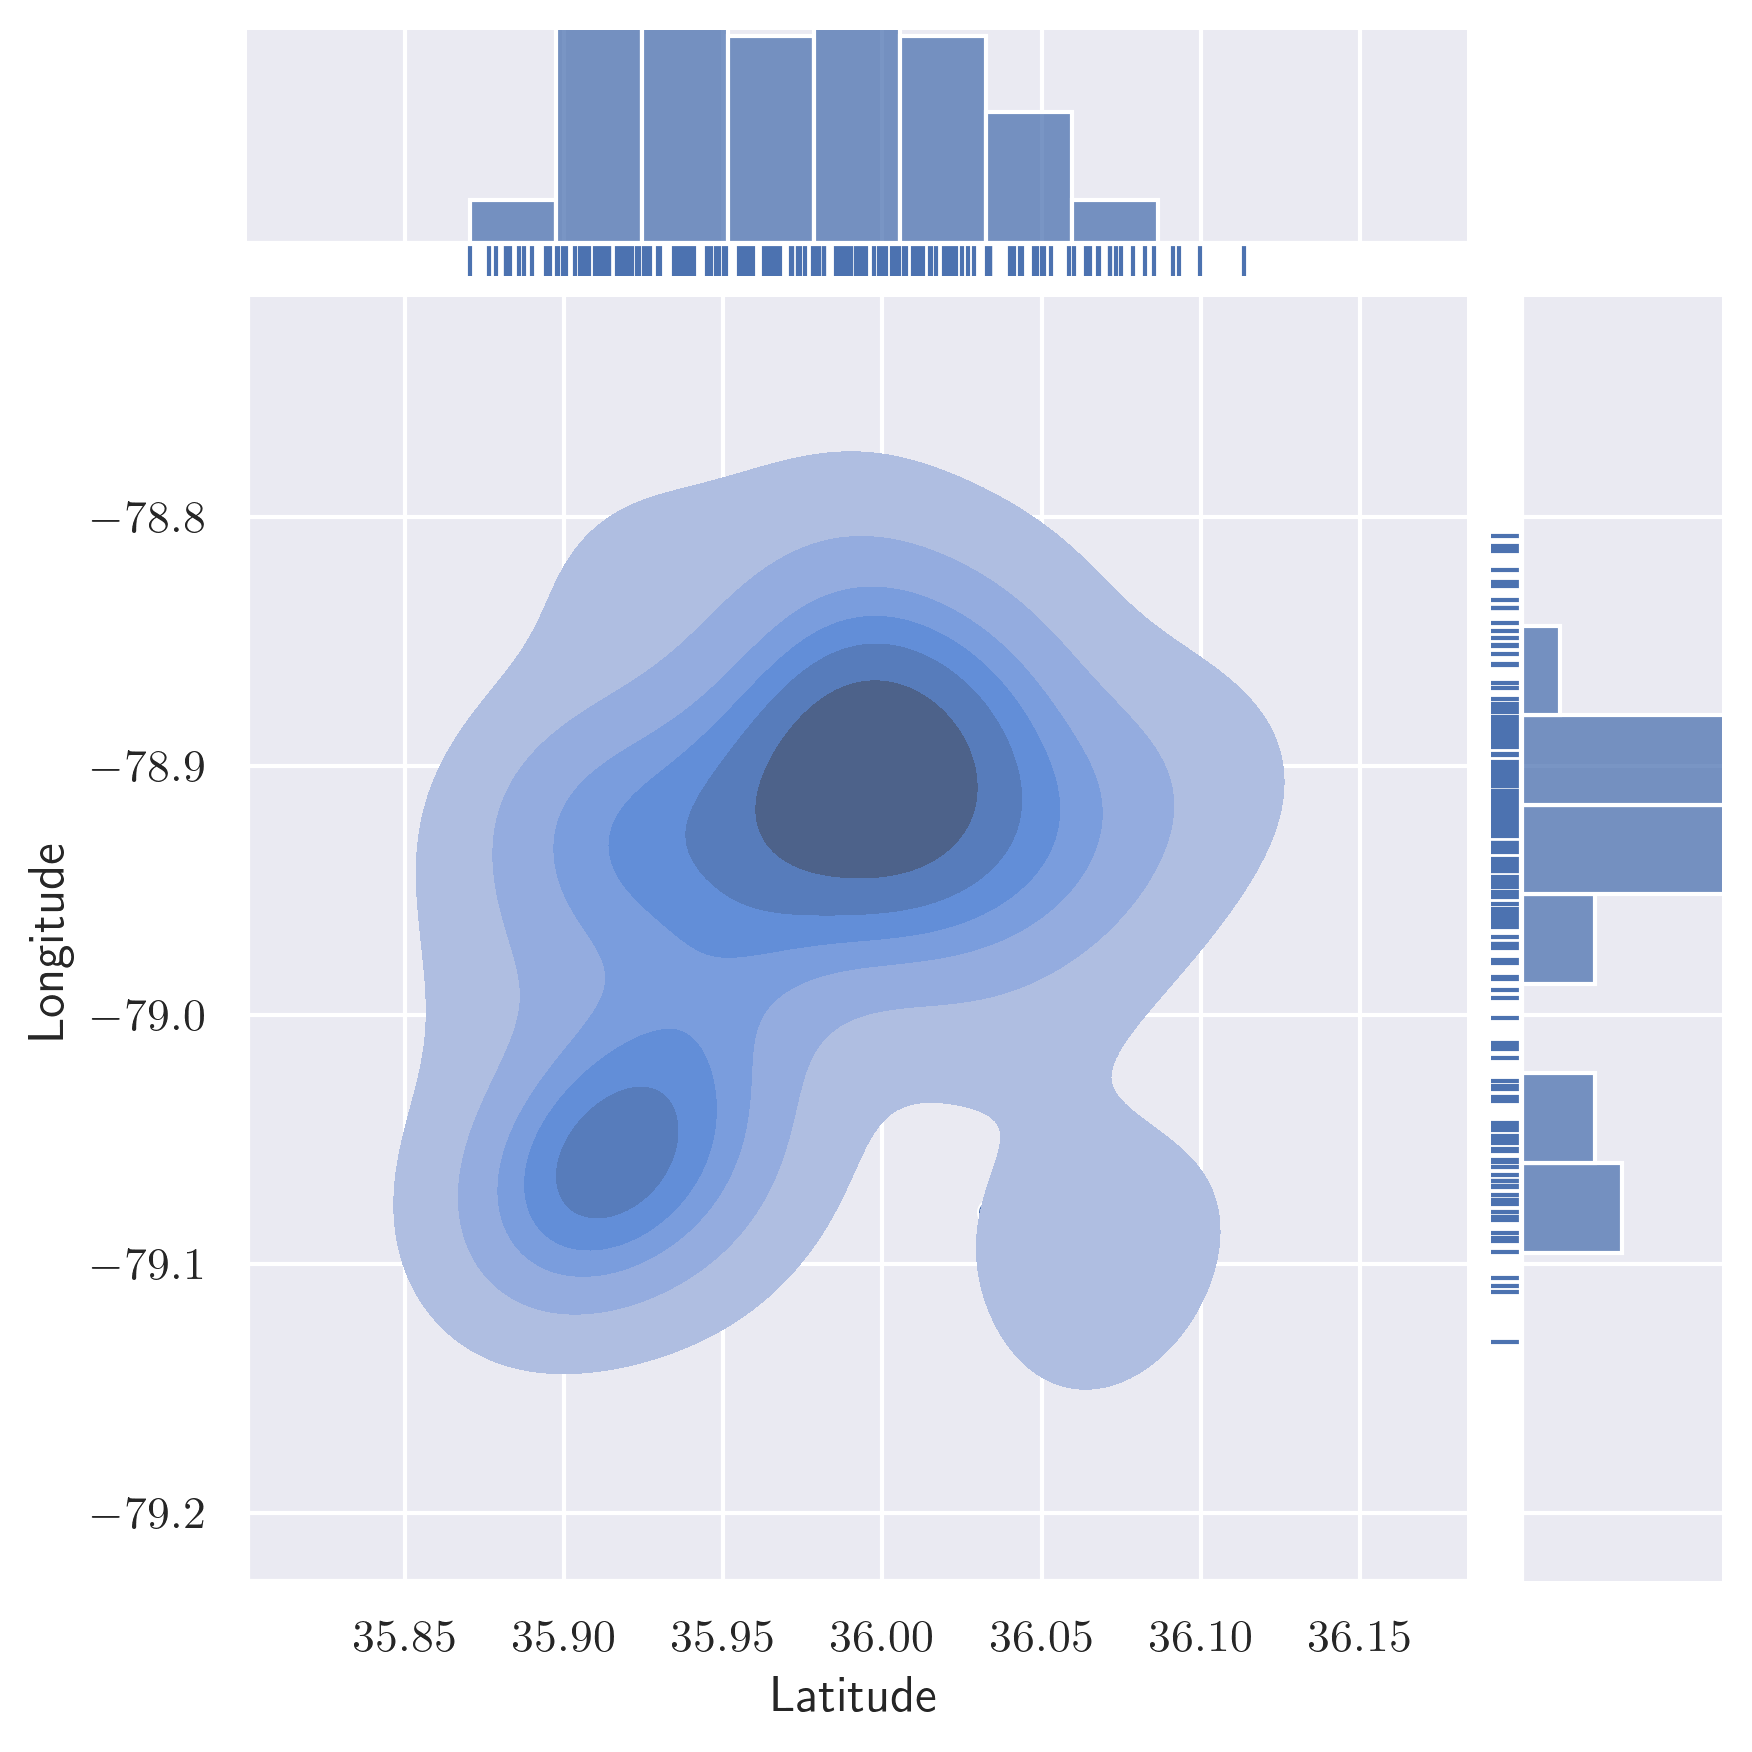
\includegraphics[width=0.9\textwidth]{Initial Analysis Images/inan_density.png}
    \caption{Tract density across the city}
    \label{fig:tract_density}
\end{figure}
Figure \ref{fig:tract_density} reveals that the coordinates mainly concentrate around two regions and are otherwise evenly spread around with smaller localized areas of concentration. These two concentrated regions are more specifically the area around $(35.92^{\circ}, -79.05^{\circ})$ and $(35.98^{\circ}, -78.90^{\circ})$. Contextualized with a map of the local area, we can note that the upper-right cluster coincides with Duke's campus and downtown Durham, whereas the lower-left cluster coincides with UNC's Chapel Hill campus.

\subsubsection{Green Space}
Next, we explore the distribution of greenery coverage over the city---the primary factor in temperature reduction and hence, UHI effects.
\begin{figure}[H]
    \centering
    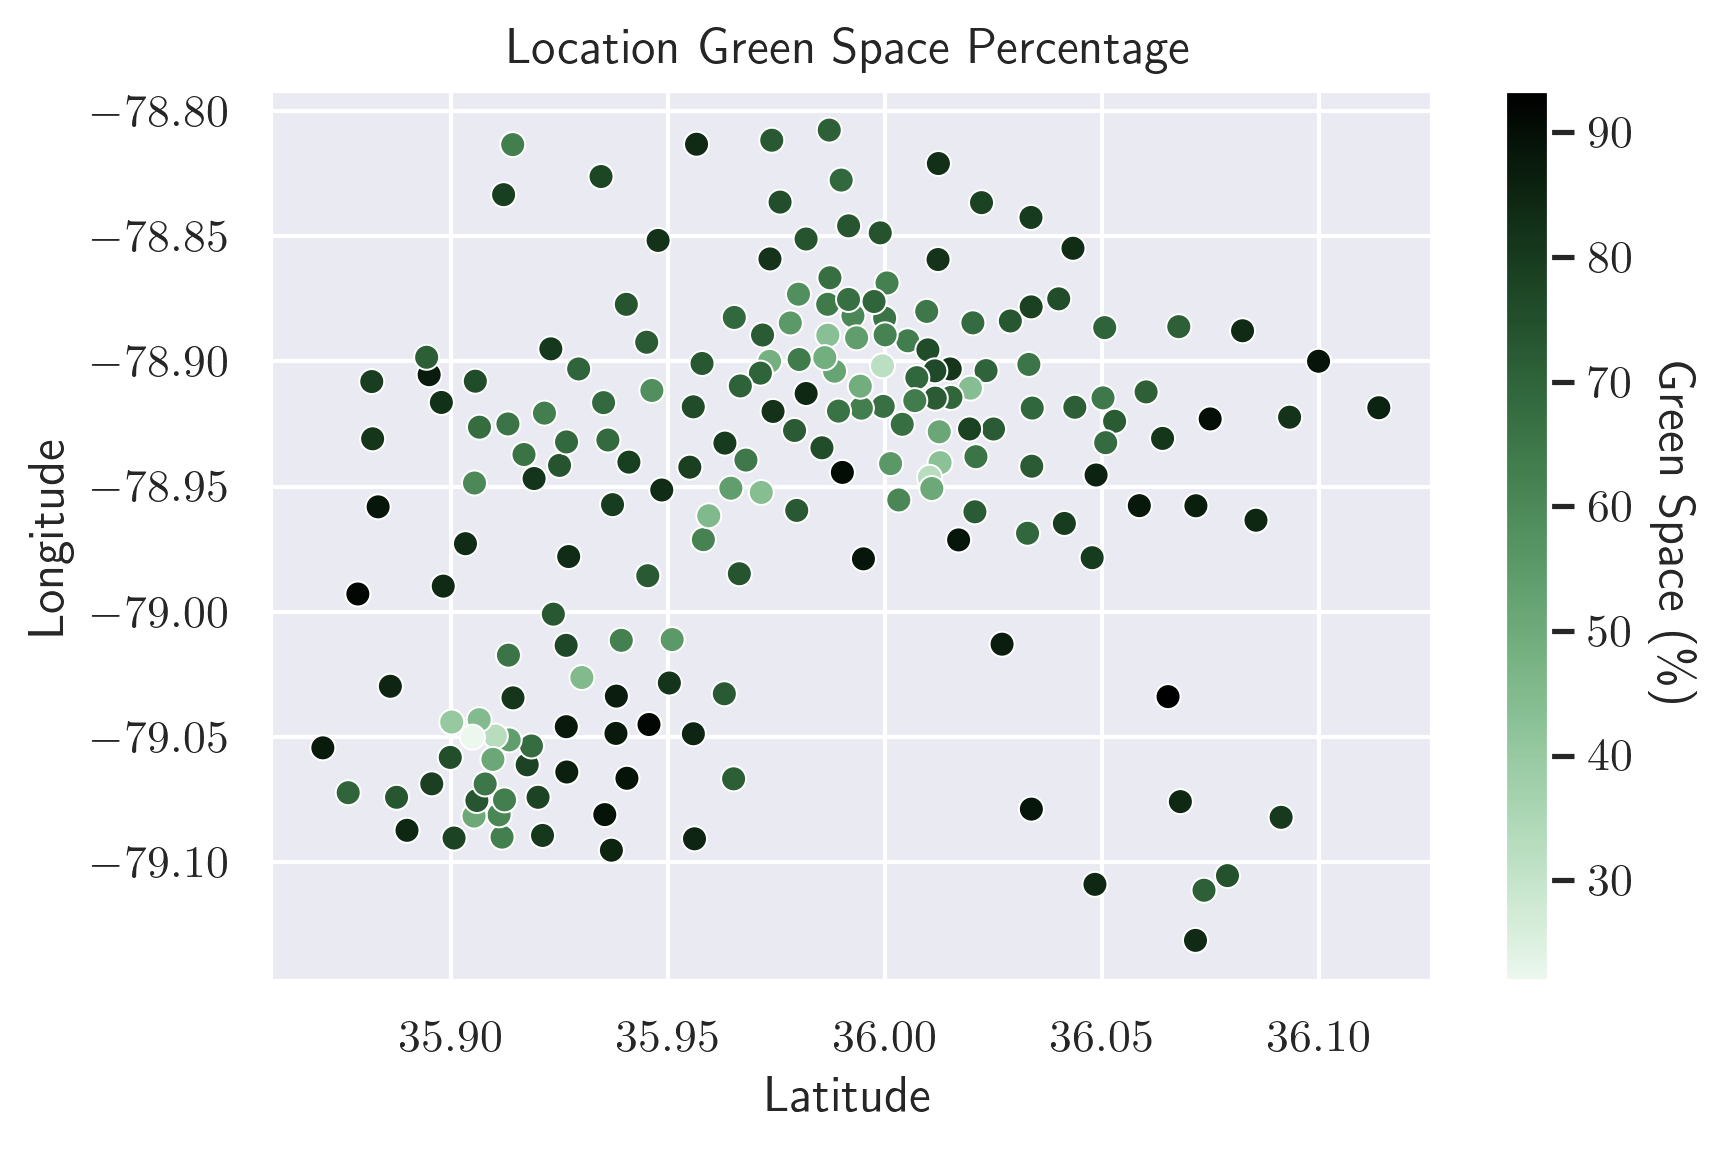
\includegraphics{Initial Analysis Images/inan_green_loc.png}
    \caption{Green space (\%) across the city}
    \label{fig:greenspace_location}
\end{figure}
From Figure \ref{fig:greenspace_location}, we observe that along the outskirts of the city, the percentage of green space is higher and around the two hypothesized population centers, the green space coverage is lower. This makes sense as cities have less space for trees and have more manmade structures that decrease this percentage.

\subsubsection{Average Temperature Reduction}
The following visualization \ref{fig:greenspacelocation} displays the distribution of the average nighttime temperature reduction across the city tracts.
\begin{figure}[H]
    \centering
    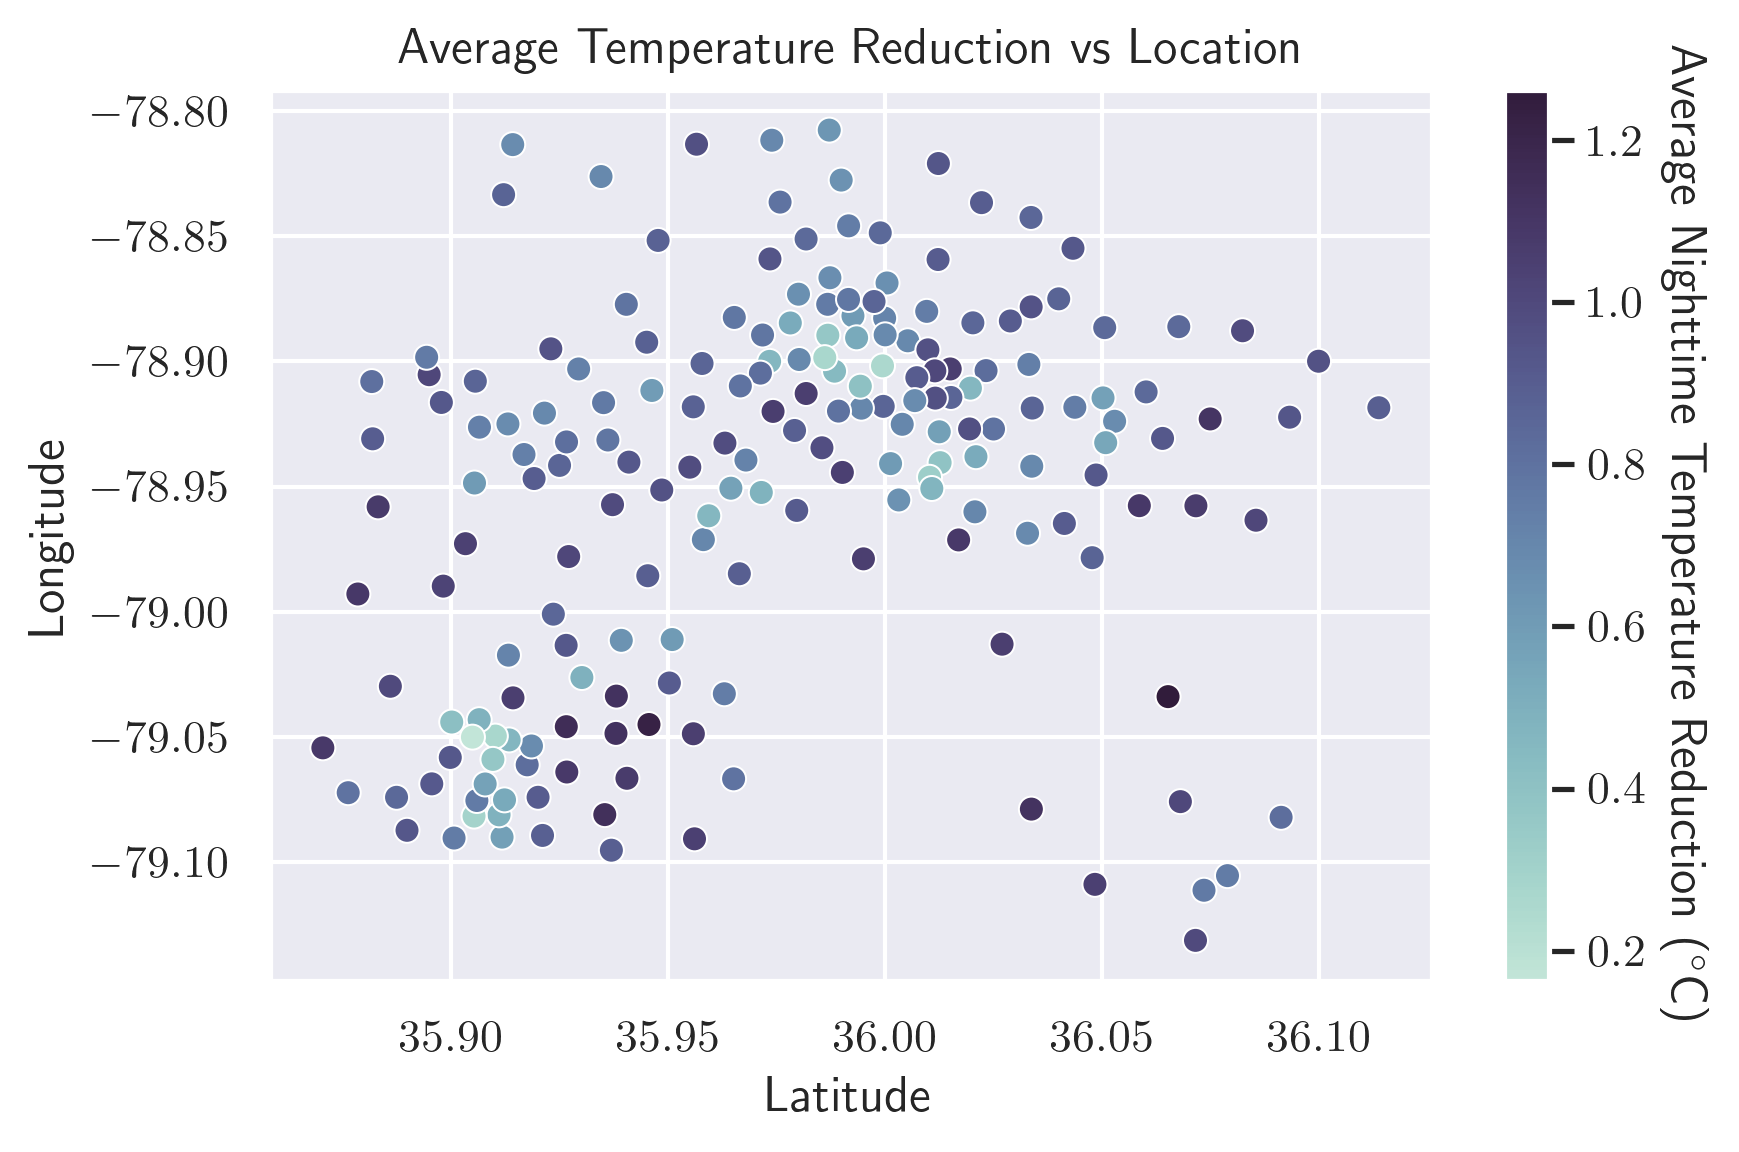
\includegraphics{Initial Analysis Images/inan_tempredux_loc.png}
    \caption{Green space (\%) across the city}
    \label{fig:greenspacelocation}
\end{figure}
Yet again, we notice the concentration of extrema in the average temperature reduction in population centers; clearly the surrounding areas are generally cooler from a larger magnitude in temperature reduction.

\subsection{Green Space and Average Temperature Drop}
From the exploration earlier, we observe that there is a relationship between green space and average temperature change; that they both take on peak values within population centers. Further analysis with an ordinary linear regression reveals a strong linear relation, with green space percentages correlating strongly with average nighttime temperature changes. Another observation is that most of the sample data points are in regions above 60\% greenery and approximately have greater than $0.6^{\circ}$C of average temperature drop.
\begin{figure}[H]
    \centering
    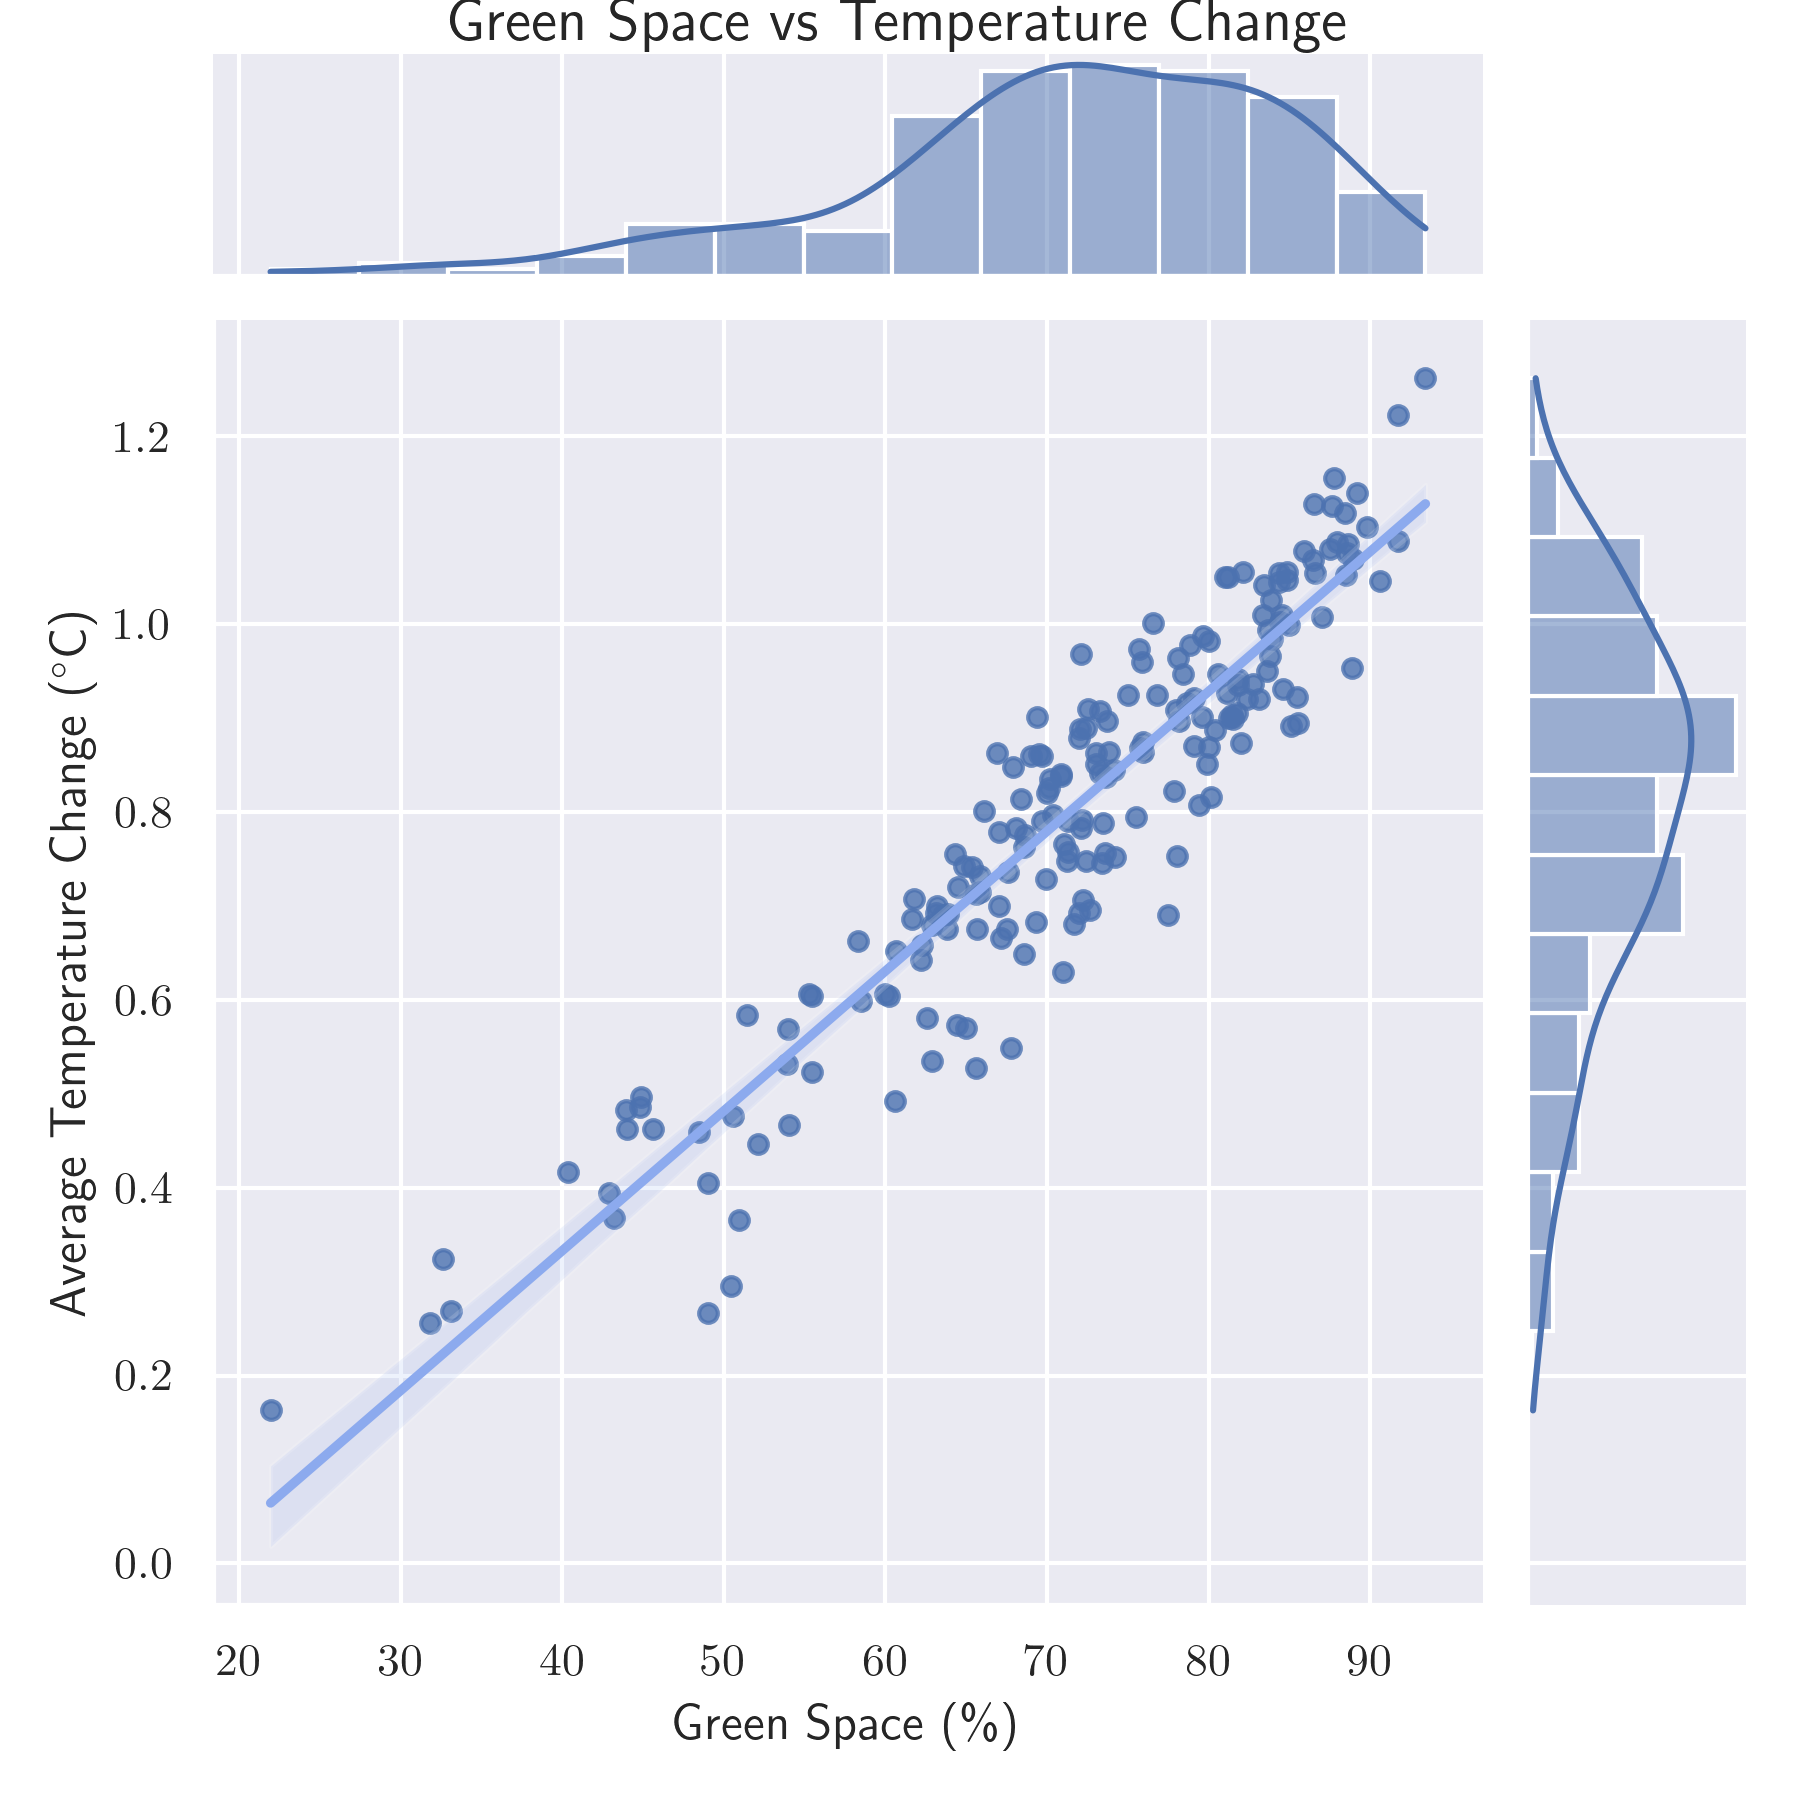
\includegraphics[width=0.7\textwidth]{Initial Analysis Images/inan_green_vs_temp.png}
    \caption{Regressing Temperature Change on Greenery}
    \label{fig:greenvstemp}
\end{figure}

\noindent The given regression line is as follows:
\begin{align}
    \hat{t} = 0.0148g - 0.26
\end{align}
where $\hat{t}$ is the predicted average nighttime temperature decrease in Celsius and $g$ is the percentage of greenery coverage. That is, for every increase in the percentage of green space, the magnitude of the average temperature drop at night increases by $0.0148^\circ C$.

This relationship can be explained by the physical role vegetation plays in temperature regulation. During the day, different surfaces absorb and hold onto heat differently. For example, materials such as concrete and roofs absorb and hold a lot more energy compared to vegetative surfaces such as grass and trees. This can be due to a variety of factors such as evapotranspiration, shading, color, etc. Critical to our modelling effort is how these surfaces release heat and alter the micro climate around city islands; that is, areas with more trees hold on to less heat and therefore releases more heat than their counterparts with less vegetation.

\subsection{Poverty}
Now we explore relations between low-income neighborhoods and UHI effects. This is because lower-income populations have less access to tools such as reliable air conditioning and healthcare. Because of this, we believe the additional utility that can be derived from planting trees in lower-income neighborhoods may be an effective strategy in maximizing the value of planting trees to reduce UHI (maximize utility). We explore relationships between poverty and measurements of green space and temperature reduction. In the following plots, we graph the percent green space and average temp change against the percent poverty of each location.
\begin{figure}[H]
    \centering
    \subfloat[\centering Poverty vs Green Space]{{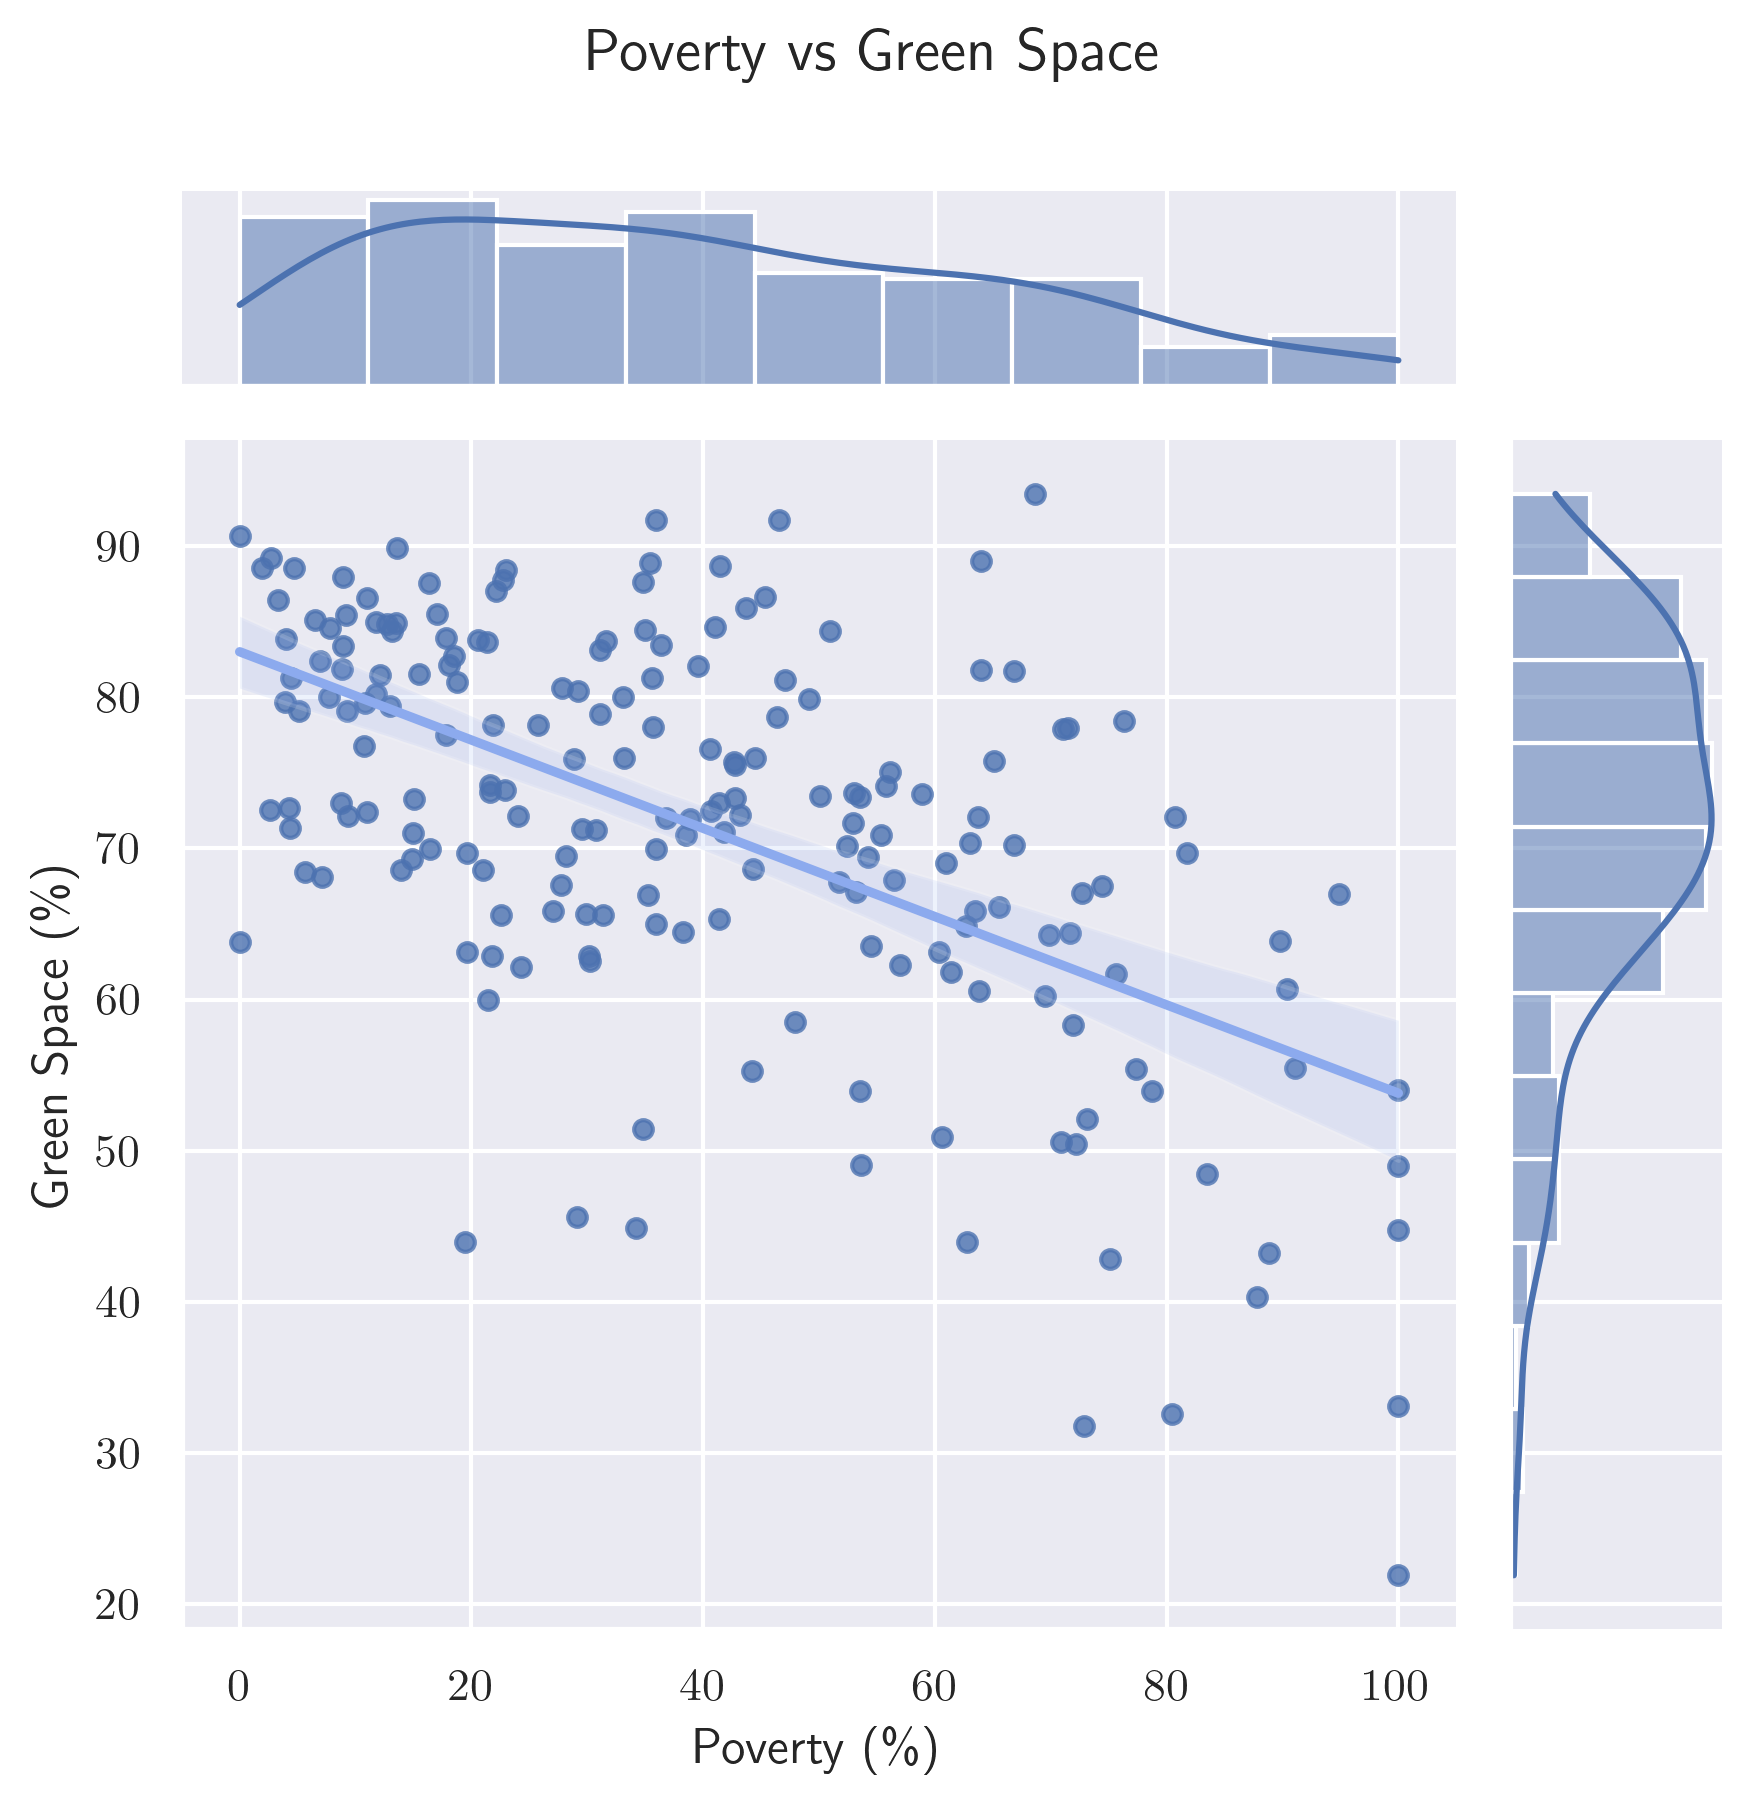
\includegraphics[width=0.49\textwidth]{Initial Analysis Images/inan_pvty_vs_green.png} }}%
    \subfloat[\centering Poverty vs Average Temperature Drop]{{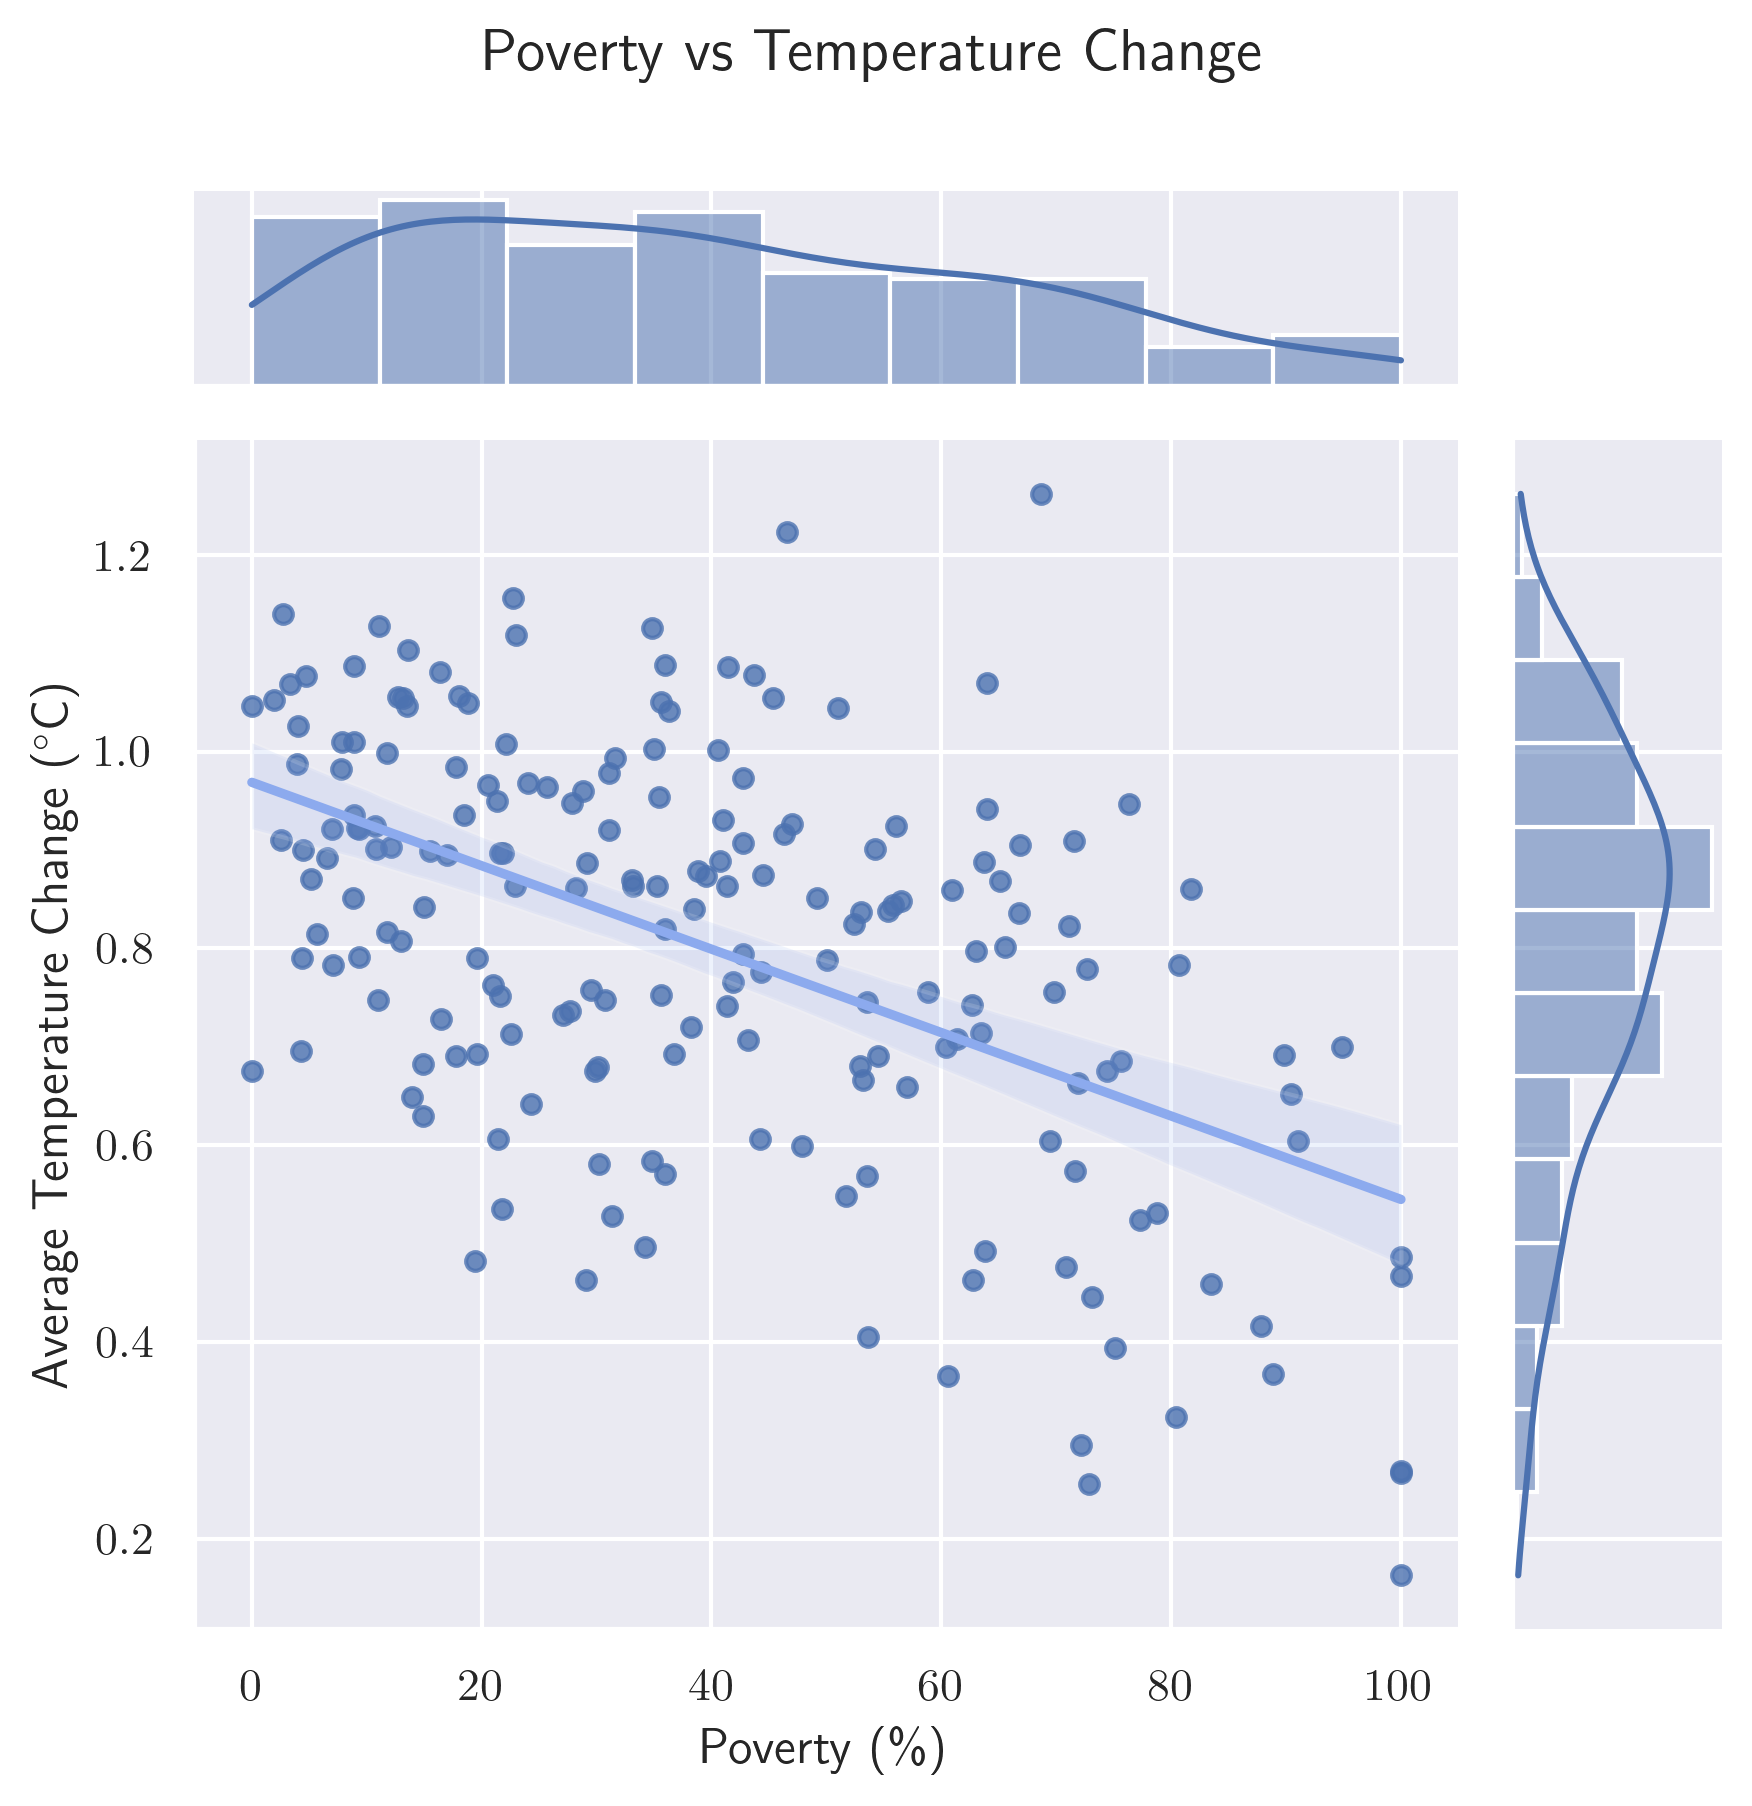
\includegraphics[width=0.49\textwidth]{Initial Analysis Images/inan_pvty_vs_temp.png} }}
    \caption{Poverty relations}
    \label{fig:fig}
\end{figure}

\subsection{Takeaways}
Below are some of the biggest conclusions we draw from our initial exploratory analysis from which we can introduce factors in modeling.
\begin{itemize}
  \item The spatial distribution of data points in the data set concentrates around two major groups that appear to be population centers
  \item Average nighttime temperature reduction has a strong positive linear relationship with green space coverage percentage.
  \item Lower income areas have less green space coverage and average temperature drop at night time, causing UHI effects to disproportionately affect the neighborhoods in question.
\end{itemize}
\pagebreak

\section{Model}
In this section, we take the findings from our initial exploratory analysis and reconcile them with our task at hand to motivate the development of a model for the mitigation of UHI effects on Durham.
\subsection{Notation}
\begin{table}[H]
    \centering
    \caption{Notation}
    \label{tab:notation}
    \begin{tabular}{cc} \toprule
        {Symbol} & {Definition} \\ \midrule
        $\mu(\cdot)$  & utility function   \\ \midrule
        $\mathcal{X}$ & set of individual tracts in Durham \\ \midrule
        $\mathcal{D}$ & set of greenery planting distribution functions \\ \midrule
        $\Delta t_{red}$  & change in average night time temperature reduction  \\ \midrule
        $\Delta x^{(s)}$ & change in greenery under $s \sim \mathcal{D}$ \\ \midrule
        $c_x$ & cost per square mile \\ \midrule
        $f$ & increment of funds \\ \midrule
        $g$ & percent green coverage \\ \midrule
        $A_x$ & area of a tract \\ \midrule
        $B$ & total budget \\ \midrule
        $\alpha$ & base cost of planting \\ \midrule
        $\lambda$ & additional cost of planting in low greenery area \\ \midrule
        $i$ & time index \\ \midrule
        $p$  & percent poverty \\ \midrule
        $\hat{t}$ & predicted average temperature drop from regression \\ \bottomrule

    \end{tabular}
\end{table}

\subsection{Motivation and Breakdown}
Our task is to quantify the effect of planting greenery on the reduction of UHI effects over time; in order to do so, we construct a model under which we can optimize the city's utility as a function of planting greenery. As we seek to analyze and mitigate the effects of UHI which can take the form of air conditioning concerns, hospitalizations, and health concerns, we chose to establish a notion of city utility as a direct measurement of UHI effects. Further, as low-income areas are disproportionately affected by UHI, we seek a metric that prioritizes balanced utility across the entire city's residents rather than one which is able to maximize utility by polarizing resource allocation. Lastly, our recommendation should be actionable and feasible---that is, we are constrained by factors such as monetary cost to the city government.

Taking these considerations into account, we present the following utility model in order to best benefit the city in relation to the  maximization of uniform city resident utility:
\begin{equation}
U_\mathcal{X} = \left( \prod_{x \in \mathcal{X}} \mu(x) \right)^\frac{1}{|\mathcal{X}|}
\end{equation}
where $x \in \mathcal{X}$ are the geographical regions (tracts) of Durham and $\mu(\cdot)$ is the governing utility function. It is apparent that we employ the geometric mean of individual tract utilities in order to discourage skewed utility maximization by asymmetric resource allocation as the geometric mean exhibits central tendency.

Then to account for the budgeting constraints that the Durham government will face in executing the greenery planting scheme, we introduce the following constraint function:
\begin{equation}
\sum_{x \in \mathcal{X}} \Delta x^{(s)} \cdot (\alpha + \lambda \mathds{1}_{\{x_{g} \leq 0.6\}}) \leq B
\end{equation}
where $\Delta x^{(s)}$ is the change in greenery percentage under some greenery planting distribution $s$ for a tract $x$, $\alpha$ is the base cost incurred by planting in a region, $\lambda$ the additional cost incurred for planting in a low greenery region, and $x_g$ is the initial greenery percentage of the region $x$. Essentially, the constraint function is the sum of the costs incurred to produce greenery percentage increases in every tract of Durham; note that there is an additional cost for planting in regions that are not sufficiently ``green".

Putting these two components together results in our final optimization problem, specified as:
\begin{equation}
\begin{aligned}
\max_{s \sim \mathcal{D}} \quad & \left( \prod_{x \in \mathcal{X}} \mu(x^{(s)}) \right)^\frac{1}{|\mathcal{X}|} \\
\textrm{subject to} \quad &\sum_{x \in \mathcal{X}} \Delta x^{(s)} \cdot (\alpha + \lambda \mathds{1}_{\{x_{g} \leq 0.6\}}) \leq B
\end{aligned}
\end{equation}
where $s \sim \mathcal{D}$ is the particular greenery planting distribution function employed.


\subsection{Assumptions}
\begin{enumerate}
    \item \textbf{Different Vegetation, Same Effect}: The model does not make the distinction that different vegetation may have different effects on the UHI effect. In reality, vegetation such as grass and shrubs do not provide the extensive shade that trees provide, their contribution to evaporation also mitigates the UHI effect. Therefore, we simplify and assume that all vegetation mitigates the UHI effect.

    \item \textbf{Financial and Infrastructural Barriers to Planting}: The model makes the assumption that the only limiting factors to increasing greenery are financial costs and the existing infrastructure in the target area. Financial constraints limit us to selecting only a small subset of regions to increase vegetation because city budgets can be limited. Infrastructure constraints make it more difficult to greenify areas with a smaller percentage of existing greenery. This is because there are additional costs such as initial soil and groundwork to develop a growing environment.

    \item \textbf{Localized Effects}: We assume that the greenery only has a localized effect on UHI. The green percent of one coordinate does not affect the average temperature drop of nearby coordinates.

    \textit{Note}: While the effects of temperature reduction are localized the utility gain may not be localized. Because the model employs a geometric mean to measure the city's overall utility, the utilities of each individual city have an effect on the utility.

    \item \textbf{Cooler Temperature, Happier Inhabitants}: The model focuses on cities with high heat so we assume that additional drops in temperature always may the inhabitants happy. We also consider any increases in average temperature drop to be negative utility.

    \item \textbf{Sustained Costs}. We assume that the entirety of the cost for planting greenery is upfront and there are no sustained maintenance costs after the planting is done.

    \item \textbf{Constant Fertility}. We assume that nothing distinguishes the fertility of a location besides the initial greenery. The model does not account for biological and geographic factors that may otherwise influence planting.
\end{enumerate}

\subsection{Additional Data}
In order to better contextualize the provided data, while also supplementing it with other key factors, we utilized US census data from \cite{census_geocoder} and \cite{mtgis}. We utilized the longitude and latitude coordinate pairings provided in conjunction with the census geocoder platform to associate the given data entries to census tract numbers. This then enabled us to enrich our data with population and area measurements for each tract obtained from the census interactive map. We believed that these two features were important considerations, the former for determining planting prioritization and the latter fro determining planting costs. Combined together, this data enabled our model to more accurately consider project efficiency, which we deemed to be critical in the context of a real-world problem.


\subsection{Change in Average Temperature Reduction at Night Time}
During the day, different surfaces absorb and hold onto heat differently. For example, materials such as concrete and roofs absorb and hold a lot more energy compared to vegetative surfaces such as grass and trees. This can be due to a variety of factors such as evapotranspiration, shading, color, etc. What is important is how these surfaces release heat at night and alter the microclimate around city islands.

Let $\hat{t}$ be the predicted average temperature reduction given a green percentage. Then the following formula is the predicted average temperature drop given that the green percentage changes from time step $i-1$ to $i$.

\begin{equation}
\begin{aligned}
\Delta t_{red} =  \hat{t}_i - \hat{t}_{i-1}
\end{aligned}
\end{equation}

\subsection{Planting costs}
Planting costs are not the same across areas with different amounts of initial greenery. Planting trees in the middle of urban cities will be more expensive because there is a lack of initial infrastructure. Planting in areas with a low percentage of green coverage likely means there are additional costs, ranging across soil work, irrigation, maintenance, etc...

To account for this, we use the following formula to describe the cost of planting trees per square mile.

\begin{equation}
\begin{aligned}
c_x = \alpha + \lambda \mathds{1}_{\{x_{g} \leq 0.6\}}
\end{aligned}
\end{equation}

As the percentage of green coverage increases past 60\%, the cost to plant becomes cheaper. Similarly, areas of low green coverage will cost more than the base price $\alpha$ because of additional infrastructural costs $\lambda$. We set our value for $\alpha$ at $500$ and $\lambda$ at $128$. This value is represented with the unit of thousands of dollars, indicating that we approximated our base cost of vegetation per square mile at \$500000 and additional cost at \$128000. We derive this number from statistics provided by \cite{satterfield_2013} and \cite{icprb_2021}, which gave estimates for tree density and planting costs, respectively. The scaled product of the estimates gave us \$250000. However, because we were not able to ascertain details regarding the planting conditions under these estimates were made, we made the assumption to let \$250000 be the cost of planting in an area with average green space ($g = 0.5$), giving an $\alpha$ of 500. Using a similar derive $\lambda$ using statistics and conversions sourced from \cite{kim_2007}.

\subsection{Effect of funds and percent green coverage}
To find the new green coverage after additional funds we use the following formula, Where $f$ is an increment of injected funds, $c$ is the cost per square mile, $g_{i-1}$ is the fraction of greenery previously, and A is the area of the region
\begin{equation}
\begin{aligned}
g_{i} = \left( \frac{\frac{f}{c_x} + g_{i-1} \cdot A_x}{A_x} \right)
\end{aligned}
\end{equation}

\subsection{Utility Function}
\subsubsection{Assumptions}
\begin{enumerate}
\item \textbf{Impoverished Neighborhoods Benefit more from UHI Reduction}.
Lower-income neighborhoods benefit more from UHI reduction than higher-income counterparts because of the law of diminishing marginal utility.
Lower-income areas have a larger number of heat-related hospitalization as well as worse access to healthcare. Mitigating UHI effects for lower-income areas should theoretically increase utility more since it deals with issues of needs instead of wants.
Additionally., high-income areas have access to reliable air conditioning, so their comfort is less sensitive to external factors such as temperature.

\item \textbf{Equal Utility Gain for Individuals}. We assume that increases in greenery increase the utility of every individual the same in a region. As a result, we assume that utility also linearly scales with population.
\end{enumerate}
The utility function captures the utility gained from planting greenery in a tract given its population, temperature reduction, percent poverty, and existing greenery.

\subsubsection{Temperature Reduction}
We assume that UHI effects are purely negative utility. Increasing the magnitude of the average temperature drop means decreasing UHI effects. Therefore actions that maximize average nighttime temperature drop $\Delta t_{red}$ increase utility $\mu_x$. Additionally, we assume that average temperature drop experiences diminishing marginal utility. Therefore we choose to represent this relationship using a natural logarithm.

\subsubsection{Percent Poverty}
The higher the percent poverty of an area, the more utility that area stands to gain from additional funds to plant trees. We assume that the relationship between poverty percentage as a decimal and utility is an exponential relationship.

\subsubsection{Population}
A larger population means there are more people to benefit from. Therefore the model attempts to capture a positive relationship between population and utility.

\subsubsection{Final Equation}
Having considered the assumptions about low-income neighborhoods, temperature reduction effects, and population, we construct the following to serve as the utility function for a single tract.
\begin{equation}
\begin{aligned}
\mu_x = S_x \times \ln(1+\Delta t_{red}) \times e^{p_x}
\end{aligned}
\end{equation}

\subsection{Optimization Algorithm}
In order to solve the optimization problem we present, we employ a pseudo-gradient descent algorithm in which funding is iteratively distributed so as to maximize the utility and obey the constraints at every iteration.
\begin{algorithm}[H]
\caption{Optimization algorithm}\label{alg:optim}
\begin{algorithmic}[1]
\State $\textrm{funds} \gets B$
\While{$\textrm{funds} >$ 0}
    \State $\texttt{curr\_util} \gets (\prod_{x \in \mathcal{X}} \mu(x))^\frac{1}{|\mathcal{X}|}$
    \State $x_i \gets \arg \max_{x \in \mathcal{X}} \Delta (U_\mathcal{X} \large|_{\textrm{Fund }x})$
    \State Allocate fund injection to $x_i$ \Comment{Inject tract with best geometric mean benefit}
    \State $\texttt{curr\_util} \gets U_\mathcal{X}'$ \Comment{$U_\mathcal{X}'$ is the geometric mean after injection}
    \State $\textrm{funds} \gets \textrm{funds} -\Delta x^{(s)}_i \cdot (\alpha + \lambda \mathds{1}_{\{x_{i, g} \leq 0.6\}})$
\EndWhile
\end{algorithmic}
\end{algorithm}
We note that our method is not a full gradient descent in the sense that we do not compute the instantaneous change in utility for each unit of funding. Rather, we break the total available funding down into increments, which we sequentially distribute to various tracts. This distribution is determined by measuring the increase in the city's utility as a whole for each offering of funds, then committing the offering to the tract which maximizes this utility increase.

We set this increment to \$10000 as a balancing point, with the consideration that perfecting the distribution down to a much greater precision is not meaningful. By this, we mean that being off by a higher precision increment, say \$100, from the supposed optimum, does not hurt the conclusions that we can derive from our model. Rather, we suggest that our model's projections are estimates, given that the actual planting of greenery is possible only in certain increments (such as the fact that planting half of a park does not make much sense).

In return for this negligible loss of accuracy, we gain a greater level of computational efficiency, which makes our model scale much better with more data. Whether that data comes in the form of optimizing funding at a federal level or at a local level with more localized temperature readings, our model will not have difficulty in giving accurate results in a timely sensible manner.


\section{Results}
\subsection{Analysis}
The results of the utility optimization algorithm are shown graphically in figure \ref{fig:density}. Most notably, we can see that the majority of tracts exhibit uniform utility with some outliers which correspond to tracts with high population density which can easily be correlated in figure \ref{fig:density}. This phenomenon is explained by the fact that the utility function is maximized by an almost-uniform allocation of greenery; however, the most densely populated areas benefit exponentially more from the greenery addition due to their marginal return rates being at their peak.

In figure \ref{fig:pvtyandutil}, we observe that most locations benefit somewhere between 0 to 10 utility points, with a few locations that benefit much more(20 to 40 utility points). Additionally, we see that the few points that have higher utility correspond to higher poverty areas.

Spatially the areas of interest for this project should be located around the coordinates $(35.92^{\circ}, -79.05^{\circ})$ and $(35.98^{\circ}, -78.90^{\circ})$.
\begin{figure}[H]
  \centering
  \subfloat[a][Tract Density]{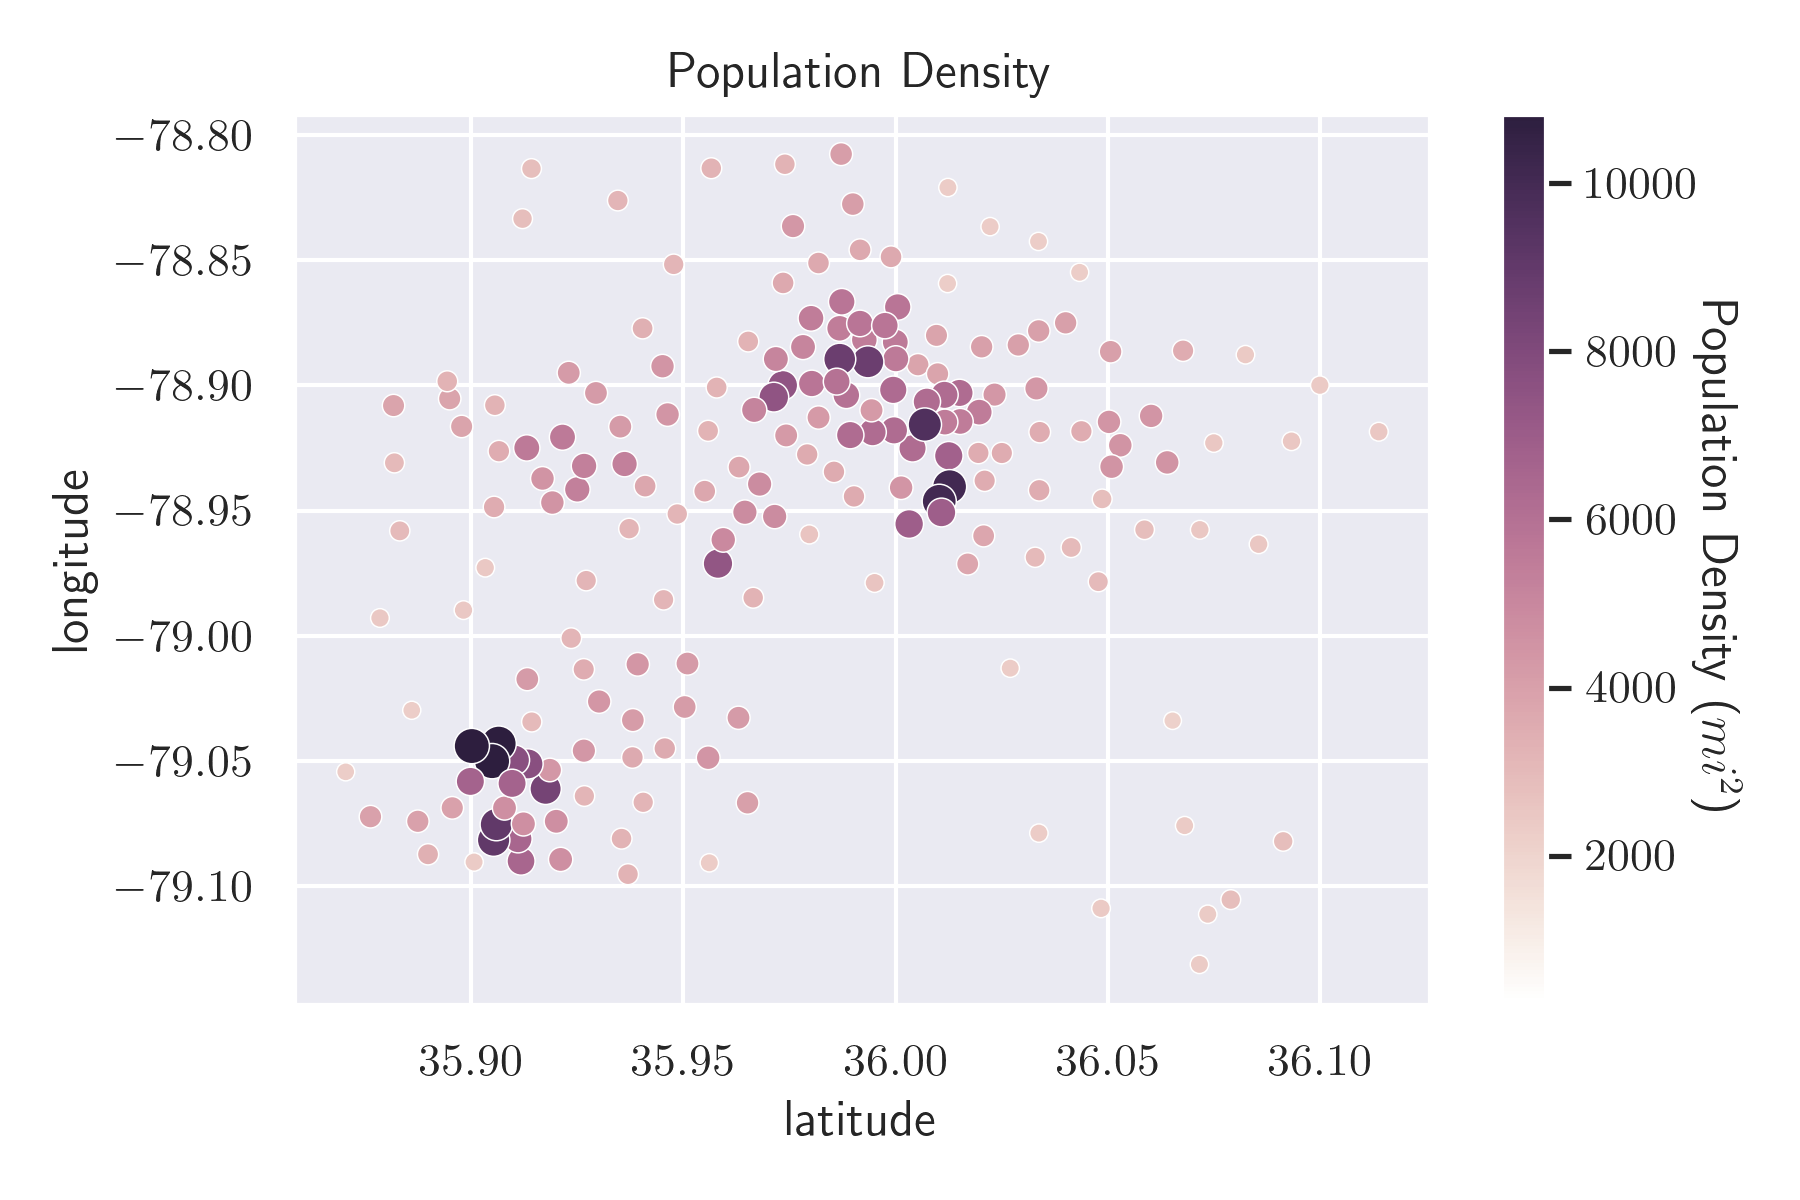
\includegraphics[width=0.7\textwidth]{Result Visualizations/viz_density.png} \label{fig:density}} \\
  \subfloat[b][Final Tract Utility]{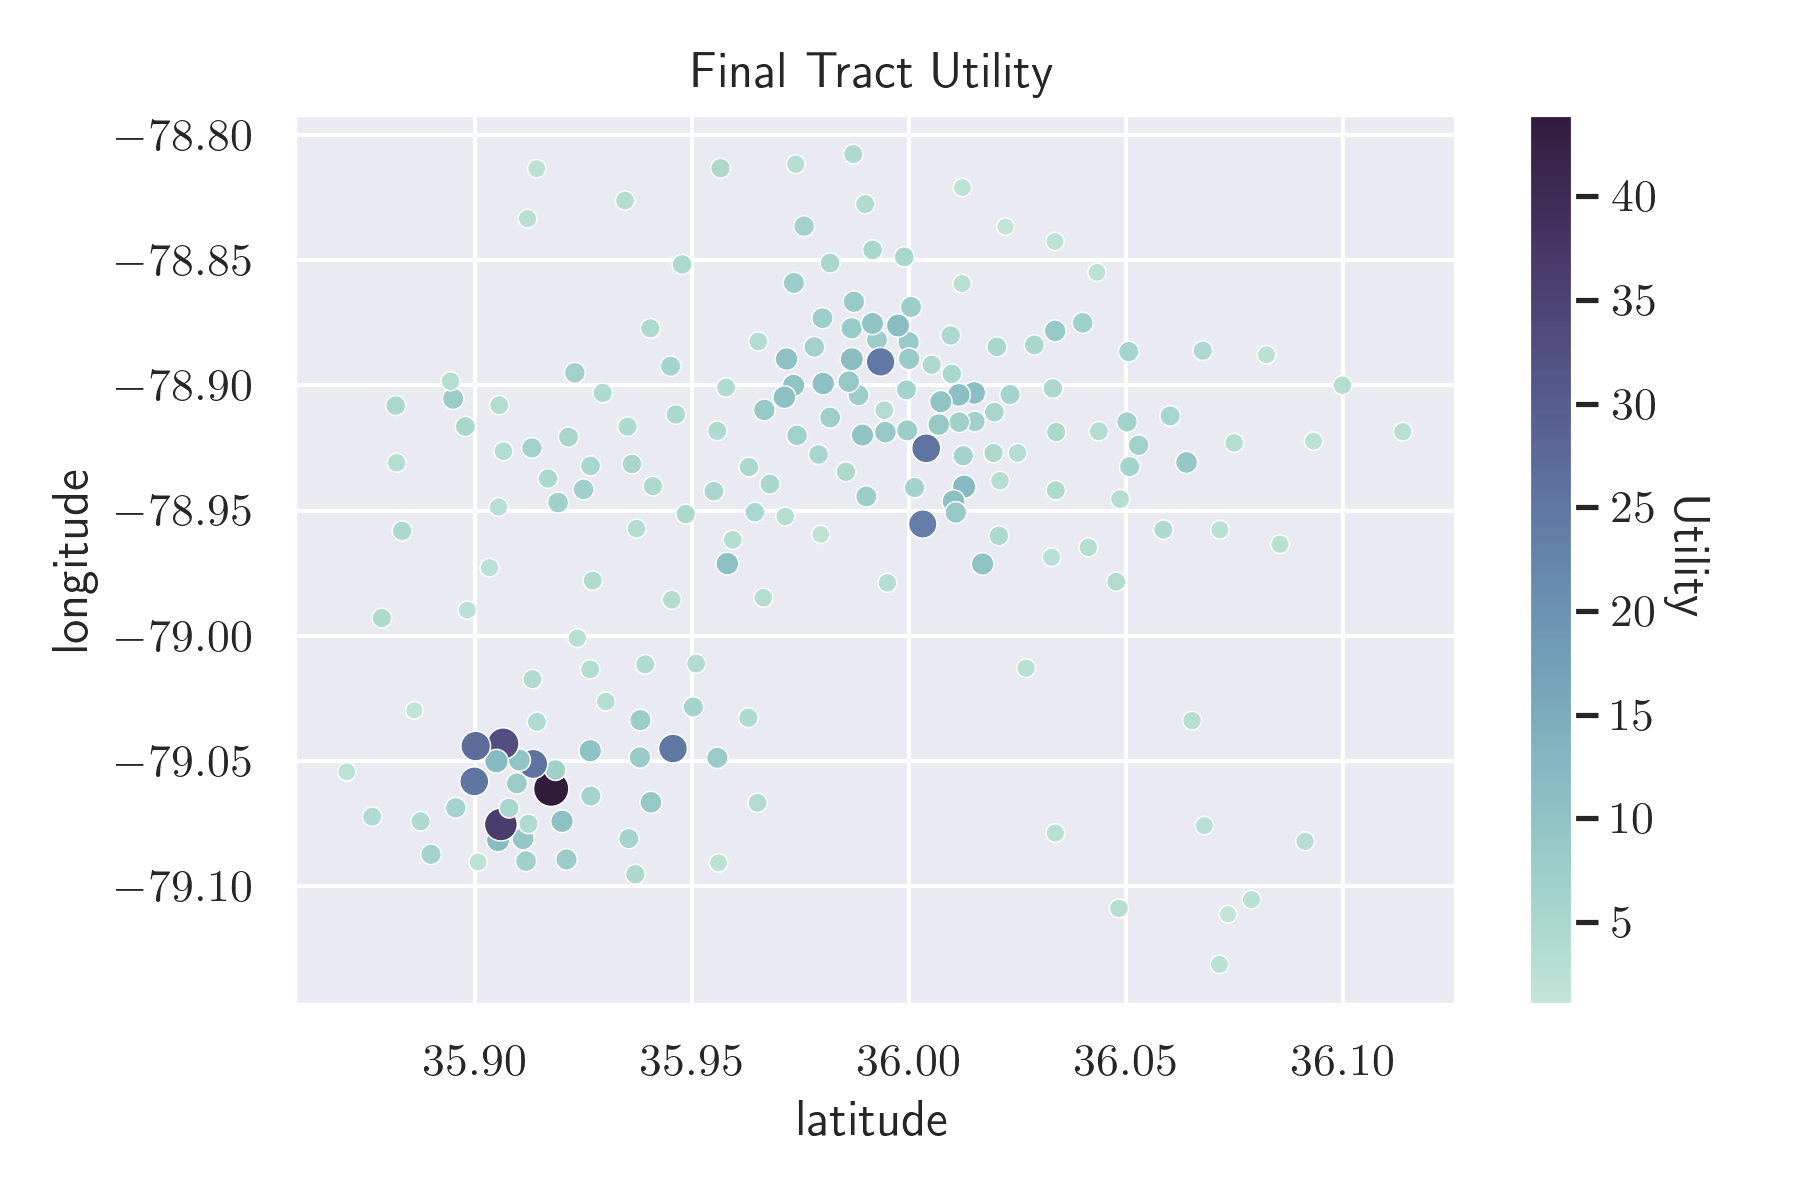
\includegraphics[width=0.7\textwidth]{Result Visualizations/viz_f_utility.png} \label{fig:utility}}
  \caption{Population Density and Utility by Tract} \label{fig:dense_utilx}
\end{figure}
Figure \ref{fig:f} displays the behavior of marginal utility over the optimization process. Clearly, there is a demonstration of diminishing marginal utility; the total utility across Durham increases over the period of 150 injections of funds for planting greenery, then the money no longer acts as efficiently---the marginal utility gain for the same amount of money begins to decrease. Assuming an initial budget of 2 million dollars and allocating funds in $\$10,000$ increments, the city of Durham should stop allocating funds at around 1.4 million after beginning to realize diminishing marginal returns in order to optimize both monetary and utility aspects simultaneously.
\begin{figure}[H]
    \centering
    {\includegraphics[width=0.7\textwidth]{Result Visualizations/viz_util_DELTA.png}} \\
    \caption{Marginal Utility across Optimization Process} \label{fig:f}
\end{figure}
Further, from figure \ref{fig:pvtyandutil} we make a rather interesting observation: most of the utility across tracts are in the $[0, 10]$ range; however, there are some outlier neighborhoods which have high final utilities. Diving deeper into this, we found that these utilities all fell outside of 2 standard deviations from the mean in final utility and corresponded to the tracts at city centers. This emphasizes the fact that the most utility is gained from allocating greenery planting efforts to the tracts which have high population density which are generally correspondent with low-income zones.
\begin{figure}[H]
    \centering
    {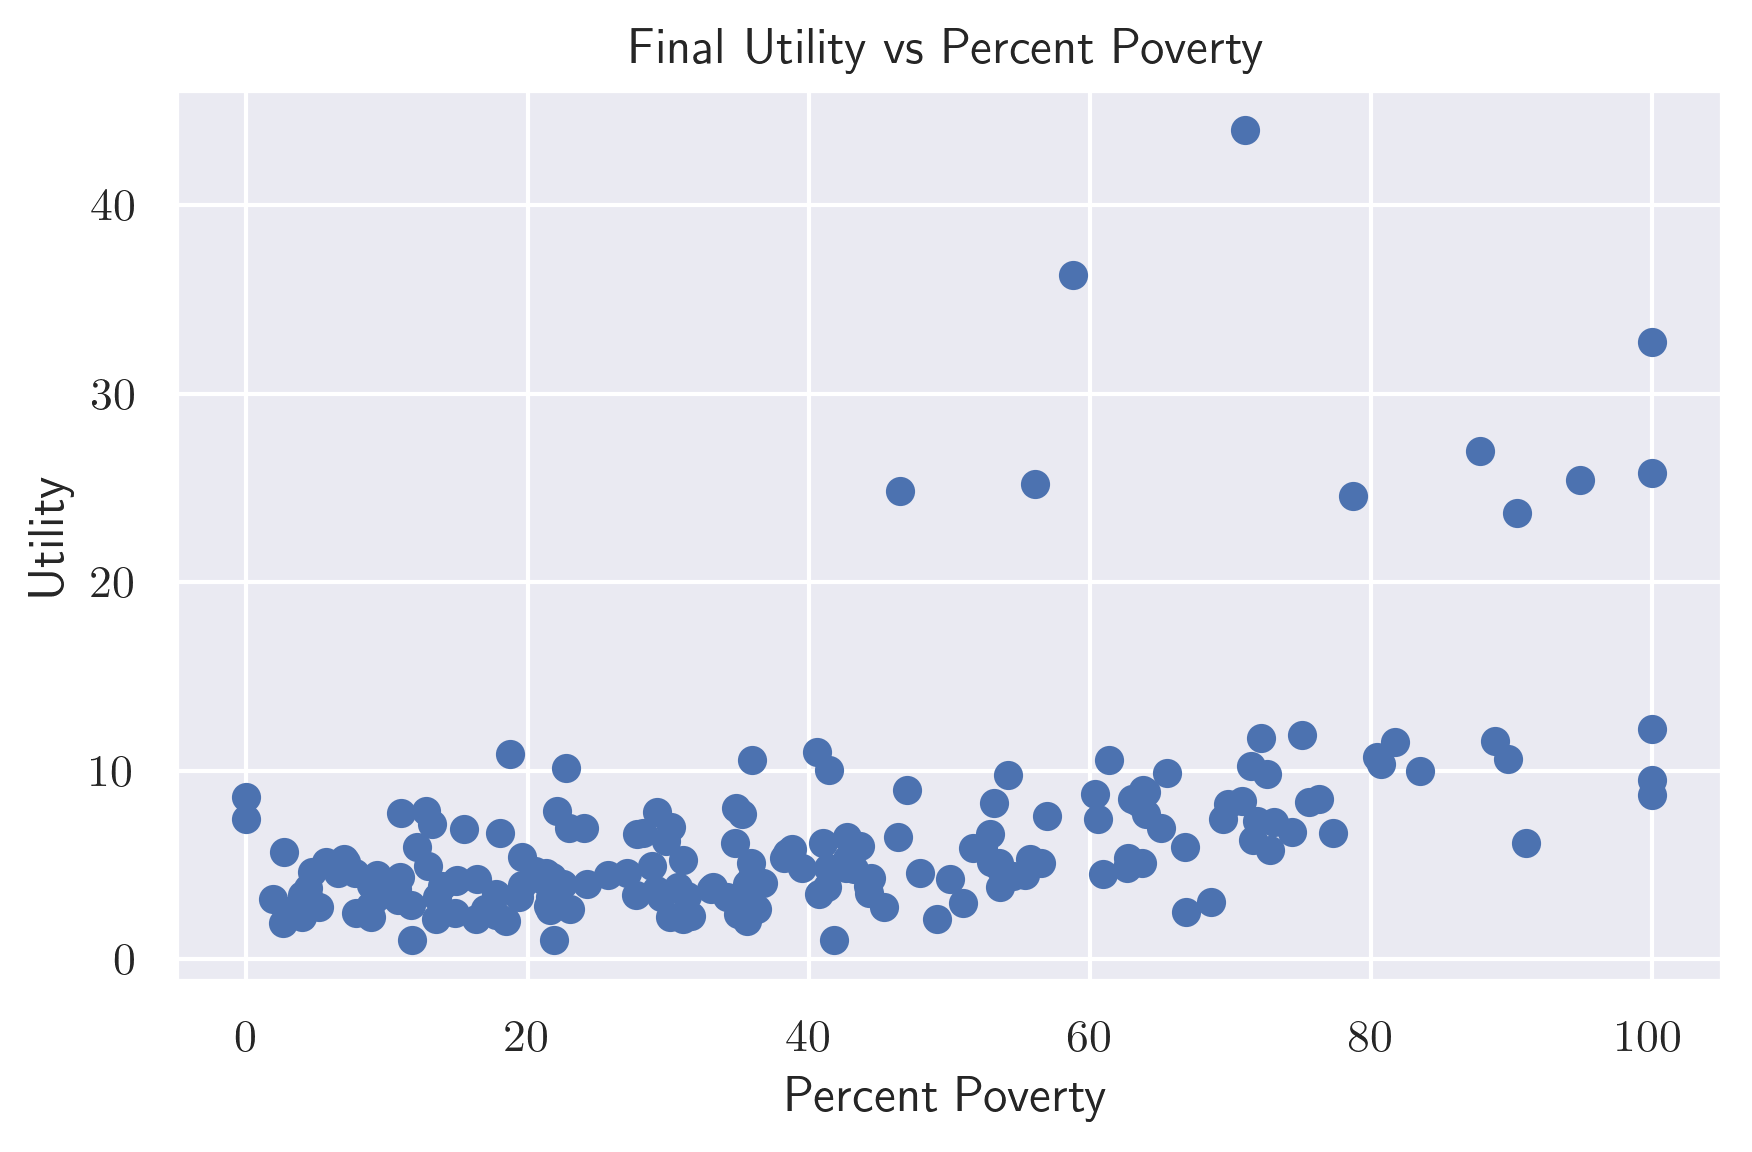
\includegraphics[width=0.7\textwidth]{Result Visualizations/viz_pvty_util.png}} \\
    \caption{Final Utility with respect to Poverty} \label{fig:pvtyandutil}
\end{figure}
\section{Strengths and Weaknesses}
\subsection{Strengths}
\begin{enumerate}
\item \textbf{Generalization}: As we have not made any constricting assumptions which only pertain to the city of Durham, our model can be generalized to any other city. Therefore, using this model, other city governments can create policies to target areas that maximize utility and social equity across the city for a variety of purposes given their individual utility and cost functions.

\item \textbf{Flexibility of Utility}: While we measure the overall utility of the city using a geometric mean, we have the flexibility to change the utility function $\mu(\cdot)$. In particular, the utility function can be changed in order to incorporate additional inputs or model different relationships between inputs. Because of this, we can create different utility functions that have different financial, environmental, or social intents.

\item \textbf{Social Equity}: Considering that one of the focuses that the city of Durham would like to address in a solution is the disproportionate impact of UHI effects on low-income neighborhoods, one of our model's strengths is that it works directly towards this goal. More specifically, the utility function which we seek to maximize is the geometric mean of all city tract utilities---this results in our model favoring providing greenery allocation to lower-income neighborhoods as their marginal utility gain under this regime is considerably greater than that of an affluent neighborhood if it were given the same allocation. As a result, the optima of this utility function imply the uniform distribution of final utility values across all neighborhoods, meaning that we prioritize increasing the utility of low-income populations prior to providing additional utility to populations that are already faring well.
\end{enumerate}

\subsection{Weaknesses}
\begin{enumerate}
\item \textbf{Interpretability}: Because the primary goal of the model is to produce explainable results that can inform policy action, interpretability is important. While having flexibility in the utility function may be a good thing to test out different utility valuations, when the number of inputs is large, the projected utilities may potentially be difficult to interpret because of the large number of variable dependencies.

However, the model remains fully effective when tasked with developing the optimal strategy for planting distribution. This is because comparisons of utility can be made without the context of a meaningful unit of measurement. This weakness applies when cities are using the model to determine whether a proposal is worth the money. However, given the difficulty of quantizing some sense of individual happiness or satisfaction, we leave this aspect of decision-making to other models developed on data better suited for such measurements.

\item \textbf{Simplifying the Impact of Trees and UHI reduction}. The addition of trees and reduction of UHI effects have extended environmental and health impacts that our model does not explicitly highlight. The addition of trees can provide improvements to air quality, stress reduction, etc. which can all increase the utility of planting trees.
\end{enumerate}

\section{Potential Improvements and Future Work}
Clearly, under a recommendation regime in which we use data to gather insights and make predictions about trends, our model can be further improved and generalized through the inclusion and use of larger datasets as well as additional relevant data. Some examples of these data include healthcare and climate trends within the tracts or similar cities such that we can better inform our modeling procedure. However, there are a couple of other improvements and directions of viable future work, which we explore in the following sections.
\subsection{Potentially Correlated Resource Basket Allocation Schemes}
Another potential area of continuation would be to research the development of utility and optimization schemes in the case where the utility is not only effected by a singular component, i.e. greenery percentage, but rather a basket of components which may or may not be correlated. This adds a new dimension of nuance in the freedom to weight priority not only across tracts, but also between products in the basket as well. Further, correlation could open doors for more efficient paths to optima that may not be achievable by the modeling of a single product; for example, the effect of choosing to employ two products, say greenery and solar panels, has a multiplicative effect on the reduction of UHI effects with only a slight increase in cost.

This expansion of research would lead to the more difficult task of optimization in high dimensions but at the benefit of much greater flexibility and applicability---rarely are governments only focusing on the effect on a single independent factor on the region; rather, there are often realistically multiple different elements which must be finely balanced.

\subsection{Robust Resource Allocation Algorithms}
A possible and applicable improvement is the development of robust resource allocation algorithms. During the collection of data for analysis, one observation we made was that some of the available government data were either outdated or poorly maintained; for example, data entries could be missing for multiple tracts. The loss or generally, corruption, of the data upon which the allocation scheme is decided would be detrimental to any practical application, particularly for cities that may not frequently maintain their data. Hence, we are interested in developing corruption-robust allocation algorithms which are guaranteed to discover global optima regardless of data poisoning. Formally, we seek to construct provably robust algorithms for optimization on $\epsilon$-corrupted data similar to the meta-algorithm for robust stochastic optimization explored in \cite{diakonikolas_2019}.

Clearly, a direct benefit of this development would be that our work could be abstracted to be useful to any city which maintains some semblance of relevant data records. Further, generally robust algorithms would go beyond just that of UHI effect mitigation; we would be able to apply it under a variety of different planning schemes ranging from park placement to road development and everything in between.

\subsection{Contextualizing the Utility Gained from Vegetation}
Our current model compares the various possible distributions of funding and greenery with the goal finding the optimum, where the utility of the city as a whole is maximized. Because we are making comparisons within the framework of the model, the fact that our model's representation of utility cannot be quantized is not problematic. However, if we are to try using the resulting utility figures to conclusively say that a project will be worth implementing at a certain cost, a roadblock is met.

Because of this, we are not able to put a hard dollar count on the value being added by the model's proposed optimal project, despite knowing that it is the best possible distribution.

Therefore, had we had more time, our team would have looked into possibly utilizing another data set to quantify utility gained in terms of a more interpretable unit. Even without it, we are able to answer important questions, but we believe that adding this element would have enabled us to give a more nuanced recommendation of a project.
\pagebreak

\section{Conclusion}
As cities around the world continue to rise and develop in an era of global warming, UHI effects can be dangerous to human health during the summer months. Additionally, UHI effects are a particular concern to low-income populations without reliable cooling and restricted access to healthcare. As a result, city governments such as Durham, NC actively seek to develop policies for planting greenery to combat UHI effects and generally, increase population health and happiness.

With the use of data sourced from the city about a variety of components such as neighborhood poverty compositions, current greenery coverage, and population, we construct a model which measures city utility as a proxy for the effects of UHI. Further, we take into consideration the importance of financial and social constraints that the city may realistically face. Coupled with this, we devise an optimization scheme in order to fully realize the effects of greenery planting on overall Durham utility and discover the best allocation for greenery which maximizes the temperature drop in the city.

Using the results from our model, we are able to geographically map out the optimal tracts to plant greenery in order to maximize the overall utility of the city. Specifically, the city of Durham should allocate approximately 1.3 to 1.5 million dollars to greenery planting efforts in the regions around coordinates $(35.92^{\circ}, -79.05^{\circ})$ and $(35.98^{\circ}, -78.90^{\circ})$.

\pagebreak

\section{Proposal to the Durham Government}
\noindent Dear Mayor Elaine O’Neal,

Our research team writes to you with the hopes of aiding the city of Durham in addressing the growing concerns over the Urban Heat Island effect. Although Durham is not the most heavily populated of cities, it nevertheless suffers from the fallout effects of global warming. We concur with the city’s recognition in that, although it may not be able to single-handedly resolve the issue of rising global temperatures, efforts can still be taken to protect the local population from its effects.

To this end, our team proposes a city-wide project to plant trees and vegetation as an endeavor to combat UHI effects. Past research by the EPA as well as other institutions indicates that increases in vegetations levels can reduce the health dangers of summer heat waves by both providing shade for heat-trapping materials such as concrete and inducing evapotranspiration processes that expedite the release of heat throughout the day. We find this to be a cost-effective plan in comparison to major green infrastructure projects. We find this to be important since our plan allows for immediate action to be taken throughout the entire city, as opposed to the decades-long rollout of expensive small-scale construction projects.

We recognize that although the city wishes to do as much as is in its power to help the residents, the resources available to be committed to this project may be limited. Therefore, we surmised, a plan of action to mitigate the effects of UHI must consider not only the effectiveness of a project, but also its efficiency. With this goal in mind, our team developed a model that works to optimize the distribution of available green funds to the various census tracts belonging to the city.

To specify, the distribution of funds created by our model emphasizes two key points.

The first is that regions with higher rates of poverty are prioritized for funding, all the while maintaining high efficiency in terms of budget-to-temperature reduction. The model does so with the recognition that the heat effects of UHI have the most severe impacts on lower-income neighborhoods with less access to insulation, air-conditioning, and regular medical care.

The second is that our model is able to account for population and area data, which allows for us to quantify more accurately the reduction in temperature achieved through a given level of funding. A distribution without these data points may struggle to consider the relative impacts of helping a large number of people at a high cost versus helping a few people at a low cost, but due to the design of our model, we are able to capture these vital comparisons and make optimal decisions.

With these considerations, our model was able to come up with a cost-efficient project designed to combat the effects of UHI in Durham. By following the model's suggestions, we are confident that with a projected budget proposal of \$1.5 million, it will be possible to add over 1800 acres of impactful greenery throughout the city. Thanks to the model’s optimization of funding distribution, this translates to an effective reduction of nighttime temperatures by slightly more than 0.8 degrees Celsius. By current standards of global warming, such a reduction would mitigate the effect of four decades of warming, making this a powerful investment which will pay dividends for many years.

Considering past expenditures by the city on green infrastructure projects, the cost of this project appears to be very much in line with what the city can afford. Furthermore, by following the recommended distributions of our model, the city will be able to strategically distribute the planting across the census tracts as to maximize the utility gain experienced by the residents of Durham.

Our team looks forward to working with the city of Durham and its residents to create a greener and healthier community. \\

\rightline{Sincerely, Team 01}

\pagebreak
\printbibliography

\pagebreak
\appendix
\section{Data}
\begingroup\tiny
\begin{longtable*}{|c|c|c|c|c|c|c|c|}
\hline
Tract & Avg Temp Reduction ($^\circ C$) & Poverty (\%) & Greenery (\%) & Longitude    & Latitude    & Population & Area ($mi^2$) \\
\hline
\hline
101   & 0.847667       & 56.50623886       & 67.91999817    & -78.88460488 & 36.02022844 & 3282       & 1.3  \\
101   & 0.907226       & 42.75788348       & 73.30000305    & -78.8838644  & 36.02885952 & 3282       & 1.3  \\
102   & 0.825103       & 52.4137931        & 70.12000275    & -78.90368904 & 36.02326272 & 4430       & 1.5  \\
102   & 0.741116       & 41.38785626       & 65.33000183    & -78.90122109 & 36.03312664 & 4430       & 1.5  \\
200   & 0.742552       & 62.67837541       & 64.83999634    & -78.88002715 & 36.00959211 & 2893       & 1.2  \\
200   & 0.690315       & 54.52436195       & 63.52999878    & -78.89177338 & 36.00522303 & 2893       & 1.2  \\
200   & 0.960217       & 28.82797732       & 75.87000275    & -78.89539737 & 36.00986406 & 2893       & 1.2  \\
301   & 0.46284        & 62.7430911        & 43.97000122    & -78.91069399 & 36.01965863 & 2644       & 0.6  \\
301   & 0.861752       & 28.18897638       & 69.48000336    & -78.9144127  & 36.01516696 & 2644       & 0.6  \\
301   & 0.967994       & 24.01574803       & 72.12999725    & -78.91467542 & 36.01156011 & 2644       & 0.6  \\
302   & 1.049724       & 18.77934272       & 81.01999664    & -78.90302361 & 36.01501127 & 3672       & 0.7  \\
302   & 1.001626       & 40.60606061       & 76.55999756    & -78.90378381 & 36.01146324 & 3672       & 0.7  \\
302   & 0.901283       & 54.21760391       & 69.40000153    & -78.9065127  & 36.00731602 & 3672       & 0.7  \\
401   & 0.791461       & 9.309791332       & 72.15000153    & -78.9270117  & 36.02498007 & 2564       & 1.3  \\
401   & 0.964205       & 25.72178478       & 78.13999939    & -78.92698965 & 36.01946431 & 2564       & 1.3  \\
401   & 0.527745       & 31.35435993       & 65.61000061    & -78.9380664  & 36.02093514 & 2564       & 1.3  \\
402   & 0.583461       & 34.79749002       & 51.41999817    & -78.92812022 & 36.01248291 & 2966       & 0.5  \\
500   & 0.699625       & 94.90131579       & 67             & -78.9251309  & 36.00395296 & 4192       & 0.8  \\
500   & 0.862927       & 35.24451939       & 66.87999725    & -78.91797012 & 35.99957401 & 4192       & 0.8  \\
500   & 0.700161       & 60.39325843       & 63.16999817    & -78.91869384 & 35.99454215 & 4192       & 0.8  \\
500   & 0.801081       & 65.52984166       & 66.11000061    & -78.91985634 & 35.98927044 & 4192       & 0.8  \\
600   & 0.887973       & 63.72575799       & 72.05999756    & -78.92759374 & 35.97914725 & 5507       & 2.7  \\
600   & 0.973152       & 42.69911504       & 75.70999908    & -78.93451135 & 35.98545882 & 5507       & 2.7  \\
600   & 1.046455       & 0                 & 90.62000275    & -78.94435096 & 35.9901614  & 5507       & 2.7  \\
700   & 0.405412       & 53.62731152       & 49.04000092    & -78.90991749 & 35.99429973 & 3701       & 1.3  \\
700   & 1.05485        & 13.1713555        & 84.33999634    & -78.91283432 & 35.98182027 & 3701       & 1.3  \\
700   & 1.056046       & 18.04961506       & 82.15000153    & -78.91998861 & 35.97419721 & 3701       & 1.3  \\
900   & 0.714413       & 63.44086022       & 65.87000275    & -78.88273371 & 35.99989799 & 1783       & 0.4  \\
900   & 0.685738       & 75.61576355       & 61.66999817    & -78.88940023 & 36.00001732 & 1783       & 0.4  \\
1001  & 0.604393       & 69.48640483       & 60.22000122    & -78.88180753 & 35.99260041 & 3879       & 0.9  \\
1001  & 0.755617       & 69.8212408        & 64.29000092    & -78.87720685 & 35.98677939 & 3879       & 0.9  \\
1001  & 0.662885       & 71.90553746       & 58.29999924    & -78.87317152 & 35.98005686 & 3879       & 0.9  \\
1002  & 0.658896       & 56.9870484        & 62.25999832    & -78.8686807  & 36.00045423 & 6140       & 1.3  \\
1002  & 0.666354       & 53.19767442       & 67.13999939    & -78.8665987  & 35.9872941  & 6140       & 1.3  \\
1002  & 0.778827       & 72.65469062       & 67.01999664    & -78.87526444 & 35.9915803  & 6140       & 1.3  \\
1002  & 0.860054       & 81.72661871       & 69.70999908    & -78.87609385 & 35.99746096 & 6140       & 1.3  \\
1100  & 0.53156        & 78.75706215       & 53.91999817    & -78.89059429 & 35.99344063 & 4151       & 0.5  \\
1100  & 0.36741        & 88.85350318       & 43.20999908    & -78.88954956 & 35.98681091 & 4151       & 0.5  \\
1301  & 0.691264       & 89.78032474       & 63.84000015    & -78.89925132 & 35.98021488 & 1432       & 0.3  \\
1303  & 0.458997       & 83.50951374       & 48.45999908    & -78.89999771 & 35.97339507 & 4052       & 0.6  \\
1303  & 0.819855       & 35.96214511       & 69.97000122    & -78.90469176 & 35.9712845  & 4052       & 0.6  \\
1304  & 0.797337       & 63.00990099       & 70.37999725    & -78.90981025 & 35.96665755 & 2781       & 0.7  \\
1400  & 0.782782       & 80.72601556       & 72.08999634    & -78.88946963 & 35.97177444 & 2746       & 0.7  \\
1400  & 0.523759       & 77.32831609       & 55.43000031    & -78.88466168 & 35.97816905 & 2746       & 0.7  \\
1501  & 0.604256       & 91.07142857       & 55.47000122    & -78.9408338  & 36.0012675  & 3430       & 1.1  \\
1505  & 0.394118       & 75.10548523       & 42.86000061    & -78.9404539  & 36.01267863 & 3951       & 0.4  \\
1505  & 0.323652       & 80.45977011       & 32.61000061    & -78.94629352 & 36.01023767 & 3951       & 0.4  \\
1504  & 0.476014       & 70.84314649       & 50.56000137    & -78.9507799  & 36.01076508 & 3033       & 0.5  \\
1504  & 0.651928       & 90.42553191       & 60.66999817    & -78.95535577 & 36.00315489 & 3033       & 0.5  \\
1503  & 0.67518        & 0                 & 63.77999878    & -78.91566928 & 36.00684428 & 1861       & 0.2  \\
1601  & 0.984319       & 17.7916234        & 83.90000153    & -78.88776574 & 36.08235058 & 6117       & 10.2 \\
1601  & 0.953767       & 35.4534005        & 88.88999939    & -78.89994653 & 36.09986231 & 6117       & 10.2 \\
1603  & 1.103366       & 13.56321839       & 89.83999634    & -78.92298932 & 36.07489442 & 6846       & 9.9  \\
1603  & 0.935656       & 8.861283644       & 81.83000183    & -78.92229571 & 36.09319282 & 6846       & 9.9  \\
1603  & 0.894654       & 17.00819672       & 85.51999664    & -78.91851126 & 36.1137441  & 6846       & 9.9  \\
1604  & 1.068514       & 3.292410714       & 86.44000244    & -78.95766979 & 36.071607   & 6655       & 9.5  \\
1604  & 1.010037       & 7.8125            & 84.54000092    & -78.96344471 & 36.08545042 & 6655       & 9.5  \\
1705  & 0.747754       & 30.74433657       & 71.22000122    & -78.9183273  & 36.04371464 & 5794       & 2.9  \\
1705  & 0.692939       & 36.76177837       & 71.98999786    & -78.94187263 & 36.03379182 & 5794       & 2.9  \\
1705  & 0.859366       & 60.9375           & 69.01999664    & -78.91864768 & 36.03390484 & 5794       & 2.9  \\
1706  & 1.085551       & 41.44775248       & 88.66000366    & -78.9713135  & 36.01694508 & 5252       & 2.3  \\
1706  & 0.706876       & 43.20407364       & 72.19999695    & -78.96008238 & 36.02069777 & 5252       & 2.3  \\
1713  & 0.869305       & 33.04410701       & 80.01999664    & -78.97840775 & 36.0477092  & 3407       & 2.6  \\
1713  & 0.682891       & 14.85549133       & 69.29000092    & -78.96864847 & 36.03282282 & 3407       & 2.6  \\
1713  & 0.901471       & 10.78838174       & 79.58999634    & -78.96473368 & 36.04130667 & 3407       & 2.6  \\
1712  & 1.087439       & 8.905852417       & 87.94000244    & -78.95762662 & 36.05857513 & 4150       & 3.6  \\
1712  & 0.922806       & 9.154383243       & 85.44999695    & -78.9453842  & 36.04860978 & 4150       & 3.6  \\
1708  & 0.838048       & 55.37563048       & 70.88999939    & -78.88613455 & 36.06766424 & 4895       & 2.5  \\
1709  & 0.868299       & 65.06666667       & 75.73999786    & -78.8750199  & 36.04000198 & 8149       & 3.2  \\
1709  & 0.94696        & 76.30878438       & 78.38999939    & -78.87823386 & 36.03365542 & 8149       & 3.2  \\
1709  & 0.835505       & 66.7867036        & 70.19999695    & -78.88652254 & 36.05059593 & 8149       & 3.2  \\
1710  & 0.840033       & 38.48372476       & 70.88999939    & -78.91219129 & 36.06013808 & 4646       & 1.5  \\
1710  & 0.57332        & 71.62162162       & 64.43000031    & -78.9145901  & 36.05021232 & 4646       & 1.5  \\
1711  & 0.926821       & 47.02495202       & 81.12000275    & -78.93076679 & 36.06392348 & 4748       & 1.5  \\
1711  & 0.680667       & 52.93141593       & 71.69999695    & -78.92392559 & 36.05288004 & 4748       & 1.5  \\
1711  & 0.548649       & 51.68674699       & 67.77999878    & -78.93246551 & 36.05082383 & 4748       & 1.5  \\
1806  & 0.897439       & 21.89086294       & 78.18000031    & -78.83660112 & 36.02221759 & 6760       & 13.7 \\
1801  & 0.90524        & 66.84350133       & 81.75          & -78.85931742 & 36.01220683 & 8293       & 17.7 \\
1801  & 0.920544       & 31.09565217       & 83.09999847    & -78.85483203 & 36.04329163 & 8293       & 17.7 \\
1801  & 0.851617       & 49.15773354       & 79.90000153    & -78.84251652 & 36.03361343 & 8293       & 17.7 \\
1802  & 0.844253       & 55.75666164       & 74.13999939    & -78.84866603 & 35.99889007 & 7548       & 3.5  \\
1802  & 0.745898       & 53.54239257       & 73.41999817    & -78.84586139 & 35.99160239 & 7548       & 3.5  \\
1802  & 0.837337       & 52.98165138       & 73.63999939    & -78.85113013 & 35.98180695 & 7548       & 3.5  \\
1802  & 0.942132       & 64.01718582       & 81.80000305    & -78.85908235 & 35.97348191 & 7548       & 3.5  \\
1806  & 0.935838       & 18.46075173       & 82.73000336    & -78.82097701 & 36.01228499 & 6760       & 13.7 \\
1810  & 0.794621       & 42.71356784       & 75.51999664    & -78.83638804 & 35.97581384 & 3550       & 1.2  \\
1811  & 0.629451       & 14.92905614       & 71.01000214    & -78.8076303  & 35.98714263 & 6378       & 2.4  \\
1811  & 0.648923       & 13.91927575       & 68.58999634    & -78.82759443 & 35.98989004 & 6378       & 2.4  \\
1808  & 0.695296       & 4.250681199       & 72.66000366    & -78.81167798 & 35.97389765 & 11498      & 7    \\
1808  & 0.966031       & 20.55114433       & 83.77999878    & -78.81326896 & 35.95656667 & 11498      & 7    \\
1809  & 0.873087       & 39.55685891       & 82.04000092    & -78.85169051 & 35.94771253 & 7316       & 4.7  \\
1809  & 0.690678       & 17.78151261       & 77.47000122    & -78.82617191 & 35.93456517 & 7316       & 4.7  \\
2007  & 0.98227        & 7.744636316       & 80.01000214    & -78.932641   & 35.96310444 & 5080       & 2.3  \\
2007  & 0.921427       & 9.288354898       & 79.08000183    & -78.94024278 & 35.94098942 & 5080       & 2.3  \\
2007  & 0.978127       & 31.08108108       & 78.86000061    & -78.942257   & 35.95501794 & 5080       & 2.3  \\
2008  & 0.950185       & 21.34502924       & 83.62999725    & -78.95137509 & 35.94855411 & 3178       & 2    \\
2008  & 0.987491       & 3.947368421       & 79.66000366    & -78.95722904 & 35.93721218 & 3178       & 2    \\
2009  & 0.776034       & 44.32907348       & 68.61000061    & -78.88244962 & 35.9652651  & 4800       & 2.8  \\
2009  & 0.863162       & 41.33333333       & 73.01000214    & -78.9008426  & 35.95783596 & 4800       & 2.8  \\
2009  & 0.874495       & 44.4588464        & 75.94000244    & -78.91815724 & 35.95581689 & 4800       & 2.8  \\
2013  & 0.920839       & 6.940700809       & 82.36000061    & -78.91640517 & 35.89778038 & 4805       & 2    \\
2013  & 1.007632       & 22.09543568       & 87.04000092    & -78.90531536 & 35.89496788 & 4805       & 2    \\
2013  & 0.807398       & 12.95210166       & 79.41999817    & -78.90805909 & 35.88174562 & 4805       & 2    \\
2015  & 0.720227       & 38.24657534       & 64.48000336    & -78.93941779 & 35.9679464  & 5328       & 1.5  \\
2015  & 0.569181       & 53.52422907       & 53.93999863    & -78.95066325 & 35.96448014 & 5328       & 1.5  \\
2015  & 0.482426       & 19.40532081       & 43.95000076    & -78.95235328 & 35.97148471 & 5328       & 1.5  \\
2032  & 0.707448       & 61.39981977       & 61.79000092    & -78.97119197 & 35.95814188 & 3320       & 0.5  \\
2031  & 0.46301        & 29.11330049       & 45.61000061    & -78.96166856 & 35.95937928 & 2201       & 0.6  \\
2030  & 1.052558       & 1.900584795       & 88.52999878    & -78.97886642 & 35.99501904 & 4354       & 5.2  \\
2030  & 0.910234       & 2.575660013       & 72.51000214    & -78.95952188 & 35.97964637 & 4354       & 5.2  \\
2029  & 0.896782       & 21.58167036       & 73.73000336    & -78.98481277 & 35.96643061 & 3774       & 2.3  \\
2033  & 0.850721       & 8.763277693       & 73.01000214    & -79.00096892 & 35.92357953 & 4293       & 2.8  \\
2034  & 0.889008       & 40.71573261       & 72.44000244    & -78.98560992 & 35.94533335 & 6052       & 4    \\
2034  & 1.009655       & 8.885163453       & 83.40000153    & -78.97795279 & 35.92711239 & 6052       & 4    \\
2019  & 1.04142        & 36.34377276       & 83.41000366    & -78.97281259 & 35.9033351  & 5134       & 7.9  \\
2019  & 1.08842        & 35.95068138       & 91.73000336    & -78.99290699 & 35.87854232 & 5134       & 7.9  \\
2019  & 1.025938       & 3.976143141       & 83.83999634    & -78.98976682 & 35.89821934 & 5134       & 7.9  \\
2020  & 1.076318       & 4.67404674        & 88.55000305    & -78.95810003 & 35.88321462 & 8403       & 6.3  \\
2020  & 0.900007       & 4.471903501       & 81.26000214    & -78.93092616 & 35.88194935 & 8403       & 6.3  \\
2021  & 0.606078       & 21.44886364       & 60             & -78.94858209 & 35.90541503 & 4604       & 2.3  \\
2021  & 0.736309       & 27.72795217       & 67.55999756    & -78.92628536 & 35.90655887 & 4604       & 2.3  \\
2022  & 0.675429       & 29.88764045       & 65.68000031    & -78.92498671 & 35.91311583 & 4524       & 1    \\
2022  & 0.692957       & 19.58708311       & 63.13000107    & -78.92066611 & 35.92153273 & 4524       & 1    \\
2023  & 0.899395       & 15.47518923       & 81.52999878    & -78.94679155 & 35.91914586 & 2837       & 0.9  \\
2023  & 0.732083       & 27.06367925       & 65.84999847    & -78.93719692 & 35.91682012 & 2837       & 0.9  \\
2024  & 0.782725       & 7.073954984       & 68.08000183    & -78.93140217 & 35.93614511 & 7058       & 1.7  \\
2024  & 0.863743       & 22.92490119       & 73.84999847    & -78.94154598 & 35.92500813 & 7058       & 1.7  \\
2024  & 0.814158       & 5.628847845       & 68.41000366    & -78.93217396 & 35.92661731 & 7058       & 1.7  \\
2025  & 0.762898       & 20.98512057       & 68.55000305    & -78.91648173 & 35.93514892 & 6410       & 2.3  \\
2025  & 0.728674       & 16.43035863       & 69.94000244    & -78.90302379 & 35.92940893 & 6410       & 2.3  \\
2025  & 0.947298       & 27.81954887       & 80.56999969    & -78.89499009 & 35.92300065 & 6410       & 2.3  \\
2026  & 0.598766       & 47.90136411       & 58.49000168    & -78.91161586 & 35.94627425 & 6831       & 2.2  \\
2026  & 0.878351       & 38.84958474       & 71.95999908    & -78.89235133 & 35.94508285 & 6831       & 2.2  \\
2035  & 0.788143       & 50.07974482       & 73.47000122    & -78.87721375 & 35.94039015 & 6682       & 3.8  \\
2036  & 0.757434       & 29.52054795       & 71.27999878    & -78.8983602  & 35.89438982 & 4307       & 2.6  \\
2036  & 0.863888       & 33.16725979       & 75.94999695    & -78.9079154  & 35.90560737 & 4307       & 2.6  \\
2038  & 0.870442       & 5.128205128       & 79.06999969    & -78.83341244 & 35.9121195  & 5724       & 4.9  \\
2038  & 0.679444       & 30.11928429       & 62.88999939    & -78.81342249 & 35.91422154 & 5724       & 4.9  \\
2200  & 0.255522       & 72.85499247       & 31.77000046    & -78.90179059 & 35.99941187 & 3177       & 0.6  \\
2300  & 0.446123       & 73.11827957       & 52.09999847    & -78.90391404 & 35.98836063 & 2434       & 0.5  \\
2300  & 0.26666        & 100               & 49.00999832    & -78.89850212 & 35.98610664 & 2434       & 0.5  \\
10707 & 0.580532       & 30.24193548       & 62.56999969    & -79.0900113  & 35.91176594 & 3363       & 0.6  \\
10707 & 0.492382       & 63.78539493       & 60.56999969    & -79.08111188 & 35.91107436 & 3363       & 0.6  \\
10708 & 0.295515       & 72.19935985       & 50.43999863    & -79.08161311 & 35.90530426 & 2603       & 0.3  \\
10708 & 0.755946       & 58.85111372       & 73.58000183    & -79.07538607 & 35.90596098 & 2603       & 0.3  \\
10710 & 0.752905       & 35.63714903       & 78.05000305    & -79.09037983 & 35.90070863 & 3335       & 6.4  \\
10709 & 0.930816       & 41.02449889       & 84.62999725    & -79.08729273 & 35.8898653  & 1955       & 1.1  \\
10705 & 0.886934       & 29.17948718       & 80.41000366    & -79.0893357  & 35.92108659 & 5036       & 1.5  \\
10705 & 0.909011       & 71.50621118       & 77.97000122    & -79.07410599 & 35.92006031 & 5036       & 1.5  \\
10705 & 0.570457       & 35.91885442       & 65.01000214    & -79.06878779 & 35.90787356 & 5036       & 1.5  \\
10705 & 0.53505        & 21.76870748       & 62.90000153    & -79.07513353 & 35.91233007 & 5036       & 1.5  \\
10706 & 0.891951       & 6.512605042       & 85.08999634    & -79.09523927 & 35.93695029 & 3668       & 2.2  \\
10706 & 1.139672       & 2.706843718       & 89.18000031    & -79.08102088 & 35.93542729 & 3668       & 2.2  \\
10904 & 1.261831       & 68.65671642       & 93.43000031    & -79.03389837 & 36.06519345 & 3673       & 16.4 \\
10902 & 1.054908       & 45.35232384       & 86.62000275    & -79.01295215 & 36.02695298 & 6584       & 12.9 \\
10902 & 1.118158       & 23.00985595       & 88.43000031    & -79.07882715 & 36.03370428 & 6584       & 12.9 \\
11001 & 0.816382       & 11.7396358        & 80.16999817    & -79.08210287 & 36.09123666 & 4733       & 4.2  \\
11002 & 1.002335       & 34.99308437       & 84.41000366    & -79.07583765 & 36.06802991 & 4291       & 8.2  \\
11001 & 0.751791       & 21.60278746       & 74.19999695    & -79.10539222 & 36.07888479 & 4733       & 4.2  \\
11002 & 0.7655         & 41.82879377       & 71.06999969    & -79.11123321 & 36.07347412 & 4291       & 8.2  \\
11002 & 0.99394        & 31.63716814       & 83.68000031    & -79.13125081 & 36.07151326 & 4291       & 8.2  \\
11106 & 1.044536       & 50.9762533        & 84.37000275    & -79.10887611 & 36.04834707 & 2471       & 3.9  \\
11208 & 1.046813       & 13.46085724       & 84.87999725    & -79.09068678 & 35.95609831 & 5245       & 10.5 \\
11207 & 0.790019       & 4.362801378       & 71.33000183    & -79.06672769 & 35.96510476 & 4599       & 1.8  \\
11206 & 0.747673       & 10.95768374       & 72.38999939    & -79.03275312 & 35.96297023 & 4184       & 1.5  \\
11206 & 0.60679        & 44.22187982       & 55.29000092    & -79.01109837 & 35.95095432 & 4184       & 1.5  \\
11300 & 0.822262       & 71.08585859       & 77.86000061    & -79.06112661 & 35.91755449 & 3132       & 0.4  \\
11400 & 1.156149       & 22.75334608       & 87.76999664    & -79.04590046 & 35.92656293 & 3893       & 1.3  \\
11400 & 0.675853       & 74.40510737       & 67.5           & -79.05360914 & 35.91853932 & 3893       & 1.3  \\
11500 & 1.050435       & 35.59742191       & 81.23000336    & -79.03439056 & 35.91428411 & 1849       & 1.4  \\
11601 & 0.467075       & 100               & 54.02999878    & -79.05119511 & 35.91340217 & 2114       & 0.3  \\
11601 & 0.269164       & 100               & 33.09000015    & -79.04965692 & 35.91021633 & 2114       & 0.3  \\
11602 & 0.486198       & 100               & 44.77999878    & -79.04309904 & 35.90649278 & 6498       & 0.6  \\
11602 & 0.162987       & 100               & 21.93000031    & -79.05008345 & 35.90494336 & 6498       & 0.6  \\
11602 & 0.416423       & 87.79495525       & 40.33000183    & -79.04404864 & 35.90016694 & 6498       & 0.6  \\
11700 & 0.365415       & 60.57951482       & 50.93999863    & -79.05896635 & 35.90965866 & 5791       & 1    \\
11700 & 0.924401       & 56.09756098       & 75.02999878    & -79.05817906 & 35.89983487 & 5791       & 1    \\
11800 & 1.069609       & 63.97790055       & 88.97000122    & -79.06651689 & 35.9405322  & 3076       & 2    \\
11800 & 1.077901       & 43.66341714       & 85.88999939    & -79.06400732 & 35.92667699 & 3076       & 2    \\
11903 & 1.055529       & 12.75862069       & 84.83000183    & -79.04872702 & 35.95583562 & 2162       & 0.7  \\
11904 & 1.222715       & 46.5392562        & 91.73000336    & -79.04503341 & 35.94561257 & 3096       & 1.5  \\
11904 & 1.125369       & 34.82972136       & 87.62000275    & -79.04858851 & 35.93800534 & 3096       & 1.5  \\
11902 & 0.903531       & 12.13235294       & 81.43000031    & -79.02845695 & 35.9503089  & 4367       & 1.6  \\
11902 & 1.127758       & 11.03038309       & 86.54000092    & -79.03369366 & 35.9380982  & 4367       & 1.6  \\
12101 & 0.642349       & 24.26653406       & 62.16999817    & -79.01141515 & 35.9392307  & 3913       & 1.3  \\
12103 & 0.712859       & 22.52934495       & 65.62000275    & -79.01733808 & 35.91323711 & 2764       & 1    \\
12101 & 0.496851       & 34.20647149       & 44.86000061    & -79.02627327 & 35.93015239 & 3913       & 1.3  \\
12102 & 0.924341       & 10.71044133       & 76.77999878    & -79.01341952 & 35.92652677 & 1543       & 0.8  \\
12201 & 0.998756       & 11.77474403       & 84.98999786    & -79.0297625  & 35.88603298 & 3084       & 7.7  \\
12202 & 0.916013       & 46.33792603       & 78.65000153    & -79.06873474 & 35.89557033 & 5449       & 2.2  \\
12202 & 0.841606       & 15.0055991        & 73.27999878    & -79.0741095  & 35.88745941 & 5449       & 2.2  \\
12202 & 0.790708       & 19.57943925       & 69.69000244    & -79.07226721 & 35.87631929 & 5449       & 2.2  \\
\hline
\end{longtable*}
\endgroup
\section{Code}
\inputminted[breaklines=True,fontsize=\tiny,python3=True,style=pastie]{Python}{source.py}
\end{document}
